\documentclass[cornellheadings,smallerheadings]{fiu}

% These declarations make latex try hard to avoid widows and orphans.
% The FIU Graduate School is very picky about these, so you may wish to
% increase these; the maximum value is 10000.
\widowpenalty=8000
\clubpenalty=8000

% This would force all pages to have the same height.
%\flushbottom

% Input macros, if you have any.
% Macros for formatting theorems, definitions, and proofs:
\newtheorem{theorem}{Theorem}[section]
\newtheorem{corollary}[theorem]{Corollary}
\newtheorem{lemma}[theorem]{Lemma}
\newtheorem{definition}[theorem]{Definition}
\newtheorem{conjecture}[theorem]{Conjecture}
\def\proof{\rm \trivlist \item[\hskip \labelsep{\it Proof.}]}
\def\endproof{\hspace{1em}{\begin{picture}(6.5,6.5)%
  \put(0,0){\framebox(6.5,6.5){}}\end{picture}}\endtrivlist}

\newcommand{\id}[1]{\mbox{\it #1}}
\newcommand{\tid}[1]{\mbox{\tt #1}}



% You may wish to put some of the title words into an \mbox{} to prevent
% latex from breaking them, for example on the signature page ii.
\title{Analysis of Eye-Tracking Data in Visualization and Data Space}
\author{Sayeed Safayet Alam}
\conferraldate{August}{2017}
\defensedate{May 12, 2017}
\advisor{Sitharama S. Iyengar}
\memberone{Mark A. Finlayson}
\membertwo{Wei Zeng}
\memberthree{Leonardo Bobadilla}
\memberfour{Golam Kibria}
\degreefield{Computer Science}
\college{College of Engineering and Computing}
\collegedean{Interim Dean Ranu Jung}
\gradschooldean{Dean Andr\`es G. Gil}

% Lets me print a subset of the chapters, while keeping the correct numbering.
%\includeonly{
%prologue,
%chap1,
%chap2,
%chap3,
%epilogue
%}
\usepackage{cite}
\usepackage{bibentry}
\nobibliography*
\usepackage{tabularx}
\usepackage{graphicx}
\usepackage{times}
\usepackage{algorithm}
\usepackage[noend]{algpseudocode}
\usepackage{amsmath}
\DeclareMathOperator*{\argmax}{argmax}
\usepackage{multirow}
\usepackage{caption}
\usepackage{rotating}

\begin{document} 

\setcounter{page}{1}
\pagenumbering{roman}
\pagestyle{plain}

% Thesis prologue: \include after \begin{document}.

% Title page
\maketitle

% Committee approval page, using the size of committee excluding the advisor.
% Note that "3" is the only supported number!
\makeapproval{3}

% Copyright page (optional)
\makecopyright

% Dedication page (optional)
\begin{dedication}
To my mother Shahin Sultana and my wife Nahid Ferdous.
\end{dedication}

% Acknowledgments (optional)
\begin{acknowledgments}
I express my heartiest gratitude to Dr. Radu Jianu who my supervisor for the first four years. He kept in touch with my even after leaving the university and invariably helped me in completing the ongoing research. Throughout the years, his enthusiasm, assistance, and foresight gave me the necessary strength to proceed through the doctoral program and finish this dissertation. 

I would like to express my sincere appreciation to my supervisor Dr.  S. S. Iyengar for his help and support during the last years of my doctoral program. I am thankful to my committee members Dr. Finlayson, Dr. Wei Zeng, Dr. Bobadilla, and Dr. Kibria for their valuable recommendations to improve this dissertation. I also thank Dr. Nipesh Pradhananga from the school of construction and Dr. Shahin Vassigh from the department of architecture at FIU for collaborating in two projects which contributed to this dissertation.

I like to thank my family members who supported me over the last five years. My mother Shahin Sultana struggled her whole life to see me successful. This dissertation would not be even possible without her love, patience, and guidance.  I could not thank enough my wife, Nahid Ferdous. She always motivated me to complete my dissertation. I am also thankful to my sister Fahrina Alam for her unconditional support over the years.  I thank my labmate, Dr. Mershack Okoe. We worked together on many projects, and my discussion with him regarding the research problems greatly benefited me in countless scenarios. 
\end{acknowledgments}

% Abstract
\begin{abstract}
Eye-tracking data is traditionally analyzed by looking at where on a visual stimulus subjects fixate, or by using area-of-interests (AOI) defined onto visual stimuli to group semantically and facilitate more advanced analyses. Recently, there is increasing interest in methods that look at what users are looking rather than where they are. By instrumenting the code that transforms a data model into visual content, gaze coordinates reported by an eye-tracker can be mapped directly to granular data shown on the screen, producing sequences of data objects that subjects viewed in an experiment. Such data collection, which is called gaze to object mapping (GTOM) or data-of-interest (DOI) analysis, can be done reliably with limited overhead and can facilitate research workflows not previously possible. Our paper contributes to establishing a foundation of DOI analyses. To this end we define a DOI data model and highlight its differences to AOI data in structure and scale; we define and exemplify a taxonomy of DOI enabled tasks; and we discuss the space of visual designs that can support this taxonomy.
\end{abstract}



% Table of Contents
\contentspage

% List of Tables (only if you have 5 or more)
\tablelistpage

% List of Figures (only if you have 5 or more)
\figurelistpage



\normalspacing
\setcounter{page}{1}
\pagenumbering{arabic}
\pagestyle{cornell}

\chapter{INTRODUCTION}
\label{chap:Intro}

\section{Motivation}
\label{sec:Motivation}
Eye-tracking is a method of reporting eye activities using specialized hardware called ``eye-trackers''. Modern eye-trackers have several capabilities. Primarily, they can locate where a user is looking on a display device (e.g. computer screens, projection screens, hand-held, and wearable displays). Albeit several types of eye-tracking applications exist, we can divide them into two categories: interactive and diagnostic. For the former (interactive), eye-tracking is used to change an interface based on a user's visual attention, such as using eye-tracking as an alternate to pointing devices ( e.g. mouse, touch interface) or text inputs. However, the latter  (diagnostic) is to describe a user's visual attention. In this dissertation, we will primarily focus on the diagnostic category of eye-tracking applications. 

Usually, a diagnostic eye-tracking study serves the purpose of quantitatively measuring people's attentional process as they solve visual tasks. It plays a major role in research fields such as human-computer interaction, cognitive sciences, and information visualization. In a typical eye-tracking experiment of this type, an eye-tracker tracks a human subject who sits in front of a computer screen which shows a visual stimulus (i.e. image, video). The eye-tracker reports and records the subject's gaze-positions on the screen. Experimenters then test their hypotheses by analyzing the collected data using visual and statistical analytic techniques. 

Presently, eye-tracking data, accumulated as a stream of 2D gaze-samples, is analyzed by one of two approaches: point-based and area of interests (AOI) -based analysis. In point-based methods, experimenters treat gaze-samples as individual points. Afterward, they relate them to the 2D stimulus shown on the screen during the experiment. In AOI-based methods, experimenters first define certain regions or areas within the analyzed stimuli. Later, they aggregate recorded gaze samples into those AOIs, which then serve as a higher-level unit of analysis.

A major limitation of these approaches is that both of them involve a significant overhead. That is, experimenters collect gaze samples as pixel coordinates and relate them to visual stimulus by either overlaying gaze-clouds on top of the stimulus image (e.g. heatmap) or by manually defined AOIs. However, if the stimulus is dynamic or interactive, then experimenters have to repeat these analysis actions for each frame of the stimulus. Such scenario makes these approaches infeasible for dynamic or interactive stimuli.

A solution presents itself with the realization that in data visualization the arrangement and layout of visual contents are known at rendering time. Hence, for visualizations with open source code, this can be instrumented so that gaze samples are related to visual contents automatically and in real-time. In other words, we can track what data objects users are viewing at each consecutive moment in time. For example, a network visualization may contain visual representations of nodes and edges. Since we know the locations of these data objects on the screen, we can map gaze samples provided by an eye-tracker to them. To exploit the analogy with the traditional AOI nomenclature, we call such eye-tracked data objects \textit{Data of Interest (DOI)}, and the entire detection and analysis process as \textit{DOI eye-tracking analysis}. 

The particularity of DOI analysis is that we can perform it in data space rather than image space. In other words, we can couple DOIs with visualization data. Thus, DOIs intrinsically contain annotations with data attributes. As a result, we can analyze DOIs on its data-derived properties, independently from visual stimuli. Hence, it will eliminate manually relating gaze samples to visual stimuli process which traditional analysis methods (i.e. point-based and AOI-based) regularly perform. Moreover, DOI analysis will support experiments of significantly longer sessions than those possible using traditional analysis approaches. Again, operating in data space will leverage DOI analysis to answer many questions that traditional analysis approaches cannot. 

\section{Problem Definition and Contributions}
\label{sec:ProblemContribution}
This dissertation makes two contributions. First, we demonstrate that collecting sufficiently accurate DOI analysis data is feasible. Second, we seek to create the foundation for DOI eye-tracking analysis (i.e. DOI analysis). We describe the contributions in Section~\ref{sec:Contribution-1} and~\ref{sec:Contribution-2}. 

\subsection{Contribution-1:Collection DOI Data is Feasible}
\label{sec:Contribution-1}
In Section~\ref{sec:Motivation}, we have introduced the idea of relating gazes with data entities in order to produce DOI data. However, we claim that such data collection is feasible. Moreover, we also claim to collect data with our method over long experimental sessions associated with dynamic and interactive stimuli, and open-ended tasks. 

We have two assumptions on the eye-tracking experiments which we intend to collect DOI data. First, the experiments must use a visualization that has computer generated visual elements. Second, source codes for generating the visualization must be open source. Hence, experimenters can implement a part of DOI-producing code to the original code. 

DOI data will consist collection of DOIs. Albeit DOIs are customizable, we assume they will contain certain information about visualization data entity, screen information, eye-tracking information, and user-specific data. However, for simplicity, we assume DOI data is time-annotated visual elements that participants viewed during such eye-tracking experiments. We call such visual elements as viewed objects. Thus, viewed objects detection is a critical component of DOI data collection.

For detecting viewed objects, we can adopt a na\"{\i}ve method from AOI analyses. The AOI's method identifies a visual object as `detected' whenever a gaze point falls on it. However, in AOI analyses, annotated AOIs are usually large and non-overlapping. Albeit the na\"{\i}ve method is sufficient for such scenario, it will not work for complex and dense visualization. For example in a real-life visualization, hundreds of distinct visual objects may occupy the screen at the same time. Again, eye-trackers can indicate only a small screen regions (e.g. approximately one inch in diameter), which users are fixating (i.e., viewing). Since such regions are likely to intersect with multiple visual objects, mapping gazes to individual objects are compelled to be an imprecise process. Moreover, DOI instrumentation should produce data that is sufficiently accurate for meaningful analyses in the context of real-life visualizations.

In our first contribution,  we have demonstrated that such DOI instrumentation is feasible. We developed a novel DOI detection algorithm. In this algorithm, we have improved upon the na\"{\i}ve AOI detection approach. We implemented it based on the hypothesis that users are more likely to view objects that are visually appealing (e.g. highlighted), or connected (physically or semantically) to previously viewed objects. If these were true, it would allow us to distinguish between potentially viewed objects, when eye-trackers detect gaze points in the vicinity of multiple objects. We have tested this hypothesis. Moreover, we have formalized the idea into our DOI detection algorithm, and evaluated its performance over the na\"{\i}ve AOI detection approach.  

In summary, we have developed a DOI detection algorithm incrementally. Moreover, we instrumented and applied the algorithm to collect DOI data from users solving real tasks in real-life visualization. Afterward, we will evaluate the reliability and effectiveness of the collected DOI data.

\subsection{Contribution-2: Formalization of DOI Data Collection and Interpretation}
\label{sec:Contribution-2}

We claim that using DOI analysis will significantly reduce human effort on analyzing eye-tracking data. However, to harness its maximum potential, we need to formalize the process of DOI analysis. We can divide the DOI analysis process into two parts: collecting data and interpreting data. We have contributed by formalizing both of the processes above. For formalizing the former, we have developed guidelines to experimenters about instrumentation methods and DOI data model. Again, formalizing the latter would require two steps. First, we will compile a list of questions that DOI data can answer. Second, we will create novel visual analytics support to answer them. 

DOIs are closely related to AOIs. Moreover, using AOIs to analyze eye-tracking is well understood, and a plethora of visualization techniques exist to support such analyses. However, we claim that using these established AOI analysis methods to understand DOI data will not be effective due to two major challenges. First, we have observed that DOI is significantly more granular and larger than data collected in traditional eye-tracking experiments. For example, using the DOI approach, we could track hundreds or thousands of DOIs over hour-long experimental sessions. Such scenarios contrast with traditional AOI methods which typically track tens of AOIs over one or two minutes. AOI methods are unlikely to handle the significantly larger volumes of DOI data. Second, DOI data can be more useful in getting insights about the semantics of the data a user explores since DOIs couple them with data attributes. Such attributes are unavailable in AOI data, and AOI methods have not been designed to explore them. Thus, AOI methods will not be sufficiently flexible to answer the new questions that DOIs can answer. 

We divide this contribution into three sub-contributions. The first sub-contribution addresses the formalization of collecting DOI data process. The latter two address the two steps of interpreting DOI data.  

\textbf{Sub-contribution 2.1:} We have contributed to \textbf{the formalization of DOI data collection} process by providing guidelines to experimenters about how to instrument visualizations and collect DOI data. We claim that DOI data can be difficult to analyze if collected data is in a clumsy format. We also provided a DOI data model to enable experimenters to produce adequately formatted DOI data. For example, in a network visualization, DOIs may be individual nodes or clusters of nodes. Usually,  links represent a single relationship among nodes. Thus, simple links are unable to represent multiple semantic relationships among DOIs. Hence, a representation of all essential relationships among DOIs to test intricate hypotheses afterward. On the other hand, testing hypotheses may become infeasible if collected DOI data is without any data model. Thus, we would need a DOI data model to facilitate experimenters. 

\textbf{Sub-contribution 2.2:} Generally, analyzers test their hypotheses by questioning their experimental data. We have \textbf{compiled the type and range of analysis queries that are askable to DOI data}. Such questions will allow researchers to understand the classes of scientific queries that the DOI methodology can support. Methodologically, we started from the formal data model devised as part of contribution $2.1$ and exhaustively identified the types of questions that the data model can support, an approach used with reliable results in the past to generate tasks-requirements for other categories of data (e.g. geographical data, temporal data). 

\textbf{Sub-contribution 2.3:} Presently, visualization is an essential tool for data analysis. For this sub-contribution, we have \textbf{explored designs of visual solutions that could facilitate DOI data analyses}. We explored existing visual techniques for analyzing AOI data. Moreover, we implemented new visualizations based on them to support the interpretation of the larger and richer DOI data. We also explored these methods and their effectiveness while collaborating with real-life researchers to answer real-life scientific questions. Specifically, we asked design requirements and feedback from collaborators at FIU and incrementally modified our designs according to their suggestions. 

\section{Related Publications}
For the accomplishment of this dissertation, we have produced the following publications:

$\bullet$ \bibentry{AJ17}.    

$\bullet$ \bibentry{Ala16}.

$\bullet$ \bibentry{Okoe14}.

\section{Outline of the Dissertation}
We discuss the background of the research of this dissertation in Chapter~\ref{chap:Foundations}. Next, we discuss feasibility and effectiveness of collecting DOI data in Chapter~\ref{chap:DOIDataCollection}. Chapter~\ref{chap:CaseStudies} describe three experiments where we collected DOI data. Again, in Chapter~\ref{chap:DOIFormalization}, we described a data model for DOI. Moreover, we also described analysis questions that are applicable for DOI data. Next, in Chapter~\ref{chap:DOIVis}, we described visual solutions to interpret DOI data. Finally, we conclude our discussion of this dissertation in Chapter~\ref{chap:Conclusion}.

\chapter{BACKGROUND}
\label{chap:Foundations}
\section{Origin of Eye-Tracking}
Eye-trackers provide a stream of gaze points based on the subtle positions changes of eye-pupils. However, the pattern of human perception reveals that stream of gaze points are not smooth trajectories. Earlier, in the 1800s, eye movements were interests affiliated to know how people read.  Javal~\cite{javal1878essai}, Lamare~\cite{lamare1893mouvements}, and  Hering~\cite{hering1879raumsinn} first discovered that people make stops while scanning through words while reading. Thus, eye-movements yield two types of gaze points: fixations, and saccades. Fixations are the points where eye stops moving for a while. On the other hand, saccades are intermediate points where eye stops for a small amount of time during switching fixations from one object to another. Edmund Huey was the first to build an eye-tracking device to track eye movement in reading~\cite{huey1908psychology}. He used lenses with small openings attached to a pointer. Later, Judd and Buswell developed an eye movement camera to capture eye motions~\cite{judd1922silent}. 

With the progress of eye-trackers, it opened paths for more research disciplines. In 1967, Yarbus correlated eye-movements with the tasks the users were given~\cite{yarbus1967eye}. Presently, Eye-tracking is a popular tool in many research domains such as psychology, neuroscience, Marketing, human-computer interaction, data visualization~\cite{Duch02}. The applications of eye-tracking technology are discussed in Section~\ref{sec:EyeTrackingApplication}.



\section{Applications of Eye-Tracking}
\label{sec:EyeTrackingApplication}
Eye-tracking technology is gradually getting more accurate, faster, and cheaper~\cite{Duch07}. Due to its availability, more research studies are adopting it as a utility. We can divide the applications of eye-tracking technology into two categories: Interactive, and Diagnostic~\cite{Duch02}. This dissertation primarily focuses on eye tracking's diagnostic role. However, we briefly discuss its interactive applications in Section~\ref{sec:EyeTrackingInteractive}. The use of eye-tracking as a diagnostic application is discussed in Section~\ref{sec:EyeTrackingDiagnostic}. 

\subsection{Eye-Tracking as an Interactive Tool}
\label{sec:EyeTrackingInteractive}
Eye movement is significantly faster than hand movements~\cite{sibert2000evaluation}. Thus, many computer-based systems have used eye-tracking as an interactive tool. Examples include using eye-tracking as an alternative to pointing devices (e.g. mouse, touch-interface) in 2D~\cite{Jacob91} and 3D~\cite{Bolt90, Tan00}, and even as a text-input device~\cite{Maj02}. However, eye-tracking is proved as ineffective compared to traditional selective devices (e.g. mouse, touch, and keyboard) due to the difficulty between view-gazes and interaction-gazes. Such case is known as the ``Midas Touch Problem''~\cite{Jacob91}. For example, a Graphic User Interface (GUI)-based system uses eye-tracking as a selective system. The system's screen contains two icons: `A' and `B'. If a user wants to select `B' but looks at `A' (view gaze) then looks at `B' (interaction gaze) then the system may find it ambiguous to decide which icon the user wants to select. To overcome this problem, Jacob proposed several solutions such as use blinks or dwell time. However, using such solutions make eye-tracking interaction slower than traditional interaction methods~\cite{Jacob91}. 

Despite being fast, eyes are not effective to control interactions. Moreover, it cannot fully serve the selective system purpose~\cite{Zha99}. However, gaze points can indicate user's intentions and displays can alter in gradual and unobtrusive nature~\cite{Jacob91, Jacob03}. Such interactive displays are labeled as ``Gaze-Contingent Displays'' (GCD)~\cite{Duch07}.  Researchers developed GCDs by changing either screen contents~\cite{Rein03, PN02} or underlying model before rendering~\cite{Dan00, OD01, ODH02, Okoe14}. 

\subsection{Eye-Tracking as a Diagnostic Tool}
\label{sec:EyeTrackingDiagnostic}
Many research user studies use eye-tracking as a diagnostic tool. The most common form of a diagnostic eye-tracking study is a user solving visual tasks by observing visual stimuli on a computer screen while an eye-tracker records the user's gaze positions. Then, analyzers process the gaze data offline to understand how the user observed the stimuli and solved the tasks~\cite{Duch07}. In this way, researchers used eye-tracking to understand how people recognize faces~\cite{Guo14, Sha14}, how attention changes with emotion~\cite{Ver13}, how diseases may affect perception~\cite{Kim14}, and how students learn from visual contents~\cite{Zaw15, May10, vGo10, Con13}.

The use of eye-tracking in data visualization research has increased with the growing popularity, accuracy, and affordability of the technology. For example, major contributions building on eye-tracking technology include the network readability study by Pohl et al.~\cite{Poh09} and Huang et al.~\cite{Hua08, Hua05}. Moreover, the study on tree drawing perception by Burch et al.~\cite{Bur11, Bur13}. As well as, the study on decision-making visualization by Kim et al.~\cite{Kim12}.

\section{Analysis of Eye-Tracking Data}
Research studies using diagnostic eye-tracking heavily depend on analyzing eye-tracking data. Studying from the literature, we divide The analysis methods for eye-tracking data into two paradigms: point-based methods and area of interests (AOI)-based methods~\cite{Bla14}. In a point-based analysis treats each of the gaze samples as a discrete point. As such, point-based analyses usually report overall gaze patterns as spatial or temporal distributions of 2D gaze coordinates over visual stimuli. The major weakness of this approach includes the requirement to show the same set of stimuli to the human subjects (i.e. users) to be comparable, and the obligation always to analyze the collected gaze data in conjunction with the 2D screen capture. Analyzing each stimulus will result in longer analysis time for larger numbers of stimuli. Moreover, analyzers have to relate gazes with the semantic contents of stimuli manually. This approach is highly ineffective in the case of interactive and dynamic stimuli.

Alternatively, analyzers often define AOIs that are relevant to their hypotheses onto a stimulus~\cite{Bla14}. The number of gaze points landing into an AOI can then be computed automatically as a proxy for users' interest in that AOI. Higher level analyses are thus possible. Examples include but are not limited to investigating reading patterns where each word is an AOI~\cite{Bey05, San04}. Moreover, to observe where and how long users look at visual regions~\cite{Coco09, Kim12}. Again, to compare interfaces utilizing AOI fixation counts and frequencies~\cite{Coletkin09}. Usually, analyzers define AOIs over stimuli manually, and the process is significantly time-consuming. Thus, the analysis process takes prolonged time with the increasing count of stimuli and visual contents within the stimuli. Moreover, the process becomes prohibitively inefficient for interactive and dynamic stimuli (e.g. video) since analyzers have to define AOIs for each frame of a video.    
  
Several solutions are proposed to overcome this weakness. One example is the automatic AOI annotations using gaze clustering algorithms~\cite{Pri00, San04, Dru14}. However, an increase of complexity of visual contents in stimuli may increase the difficulty of the AOI annotation process. Stellmach et al. proposed the object of interests (OOI) concept for 3D stimuli where eye-trackers collect gaze points on the surface of 3D objects available in a scene~\cite{Ste10}. Additionally, Steichen et al.~\cite{Ste13} and Kurzhal et al.~\cite{Kur14} suggested the possibilities of dynamic AOI annotation in the case of computer generated visual contents. However, this concept is still unexplored. This dissertation leverages this concept of dynamic AOI and OOI into developing DOIs. We discuss related works about DOIs in Section~\ref{sec:RelatedWorks}.

\section{Related Works}
\label{sec:RelatedWorks}
Our contributions in this dissertation primarily explore the eye-tracking data collection and interpretation. We discuss related works about them in the following sections.

\subsection{Eye-Tracking Data Collection} 
In Section~\ref{sec:ProblemContribution}, we mentioned Data of Interests (DOI) as an improved solution for eye-tracking data analysis. The idea of DOI originates from the objective of automatically detecting which data objects a user of a visualization views. As such, DOI is the mapping of gaze samples to data objects rather than pixel positions. Recently, Sundstedt et al.~\cite{Sun13} and Bernhard et al.~\cite{Bern14} introduced a process called gaze to object mapping (GTOM) for identifying objects which are targets of users' attentions in 3D virtual environments. This dissertation contributes a similar approach to in the context of relating gaze points with semantic contents of network diagram~\cite{Okoe14}. However, relating gaze points with semantic contents of any visualization is non-existent. Salvucci et al. presented a probabilistic approach to predict viewed objects on a computer screen using eye-tracking~\cite{Sal00}. Moreover, Salvucci et al. alongside with Okoe et al.~\cite{Okoe14} indicated that leveraging semantics of visual contents can significantly improve viewed-object predictions. However, both Salvucci et al.'s and Okoe et al.'s contributions were limited to simple visualizations. Salvucci et al. tested their methods over a simple gaze-added WIMP (i.e. Window, Icon, Menu, and Pointer) interface. On the other hand, Okoe et al. explored only network visualization~\cite{Okoe14}. The idea of OOI and GTOM significantly influenced our first contribution. Moreover, One of our methods innovates on existing techniques for mapping gazes to objects by adopting the probabilistic method by leveraging semantic contents of visualizations.  


\subsection{Eye-Tracking Data Interpretation}
Many methods exist to interpret eye-tracking data visually. Blascheck et al. categorized several existing visualization techniques for point-based and AOI-based visualizations~\cite{Bla14}. More complex visual analytics software systems and solutions include those by Andrienko et al.~\cite{And12}, Weibel et al.~\cite{Wei12}, Kurzhal et al.~\cite{Kur14}, and Blascheck et al.~\cite{Bla16}.

However, DOI data can be significantly more granular and larger than AOI data. Moreover, we can associate DOIs with a wealth of directly-derived data attributes from the tracked data. Hence, we hypothesize that DOI data can answer questions that AOI cannot. Moreover, data interpretations using traditional AOI analysis methods are ineffective for DOI data. This shortcoming motivated our second contribution, with its two sub-goals: determining what questions DOI data can answer that AOI cannot, and creating support for theses questions. 
 
To accomplish the former, we formalized the DOI specific analytical tasks. Any specific categorizations of analysis tasks for eye-tracking data are currently non-existent. However, task categorization, task taxonomies, and task frameworks do exist for other types of data and analyses. For example, Wehrend and Lewis~\cite{Weh90}, Shneiderman~\cite{Shne96} discuss general features of task taxonomies in the context of data visualization. Recently, Brehmer et al.~\cite{Bre13}, Schulz et al.~\cite{Sch13}, and Rind et al.~\cite{Rind15} proposed a multilevel typology that can be applicable for creating complete task descriptions regardless of domain specifications. Amar et al. provided a comprehensive categorization of low-level tasks~\cite{Ama05}. Moreover, task taxonomies exist for several specific types of data visualizations such as for graph visualization~\cite{Lee06}, group level graphs~\cite{Sak14}, multidimensional data visualization~\cite{Ward02}, and geo-temporal data~\cite{And03, Roth13}. Hence, as a part of our second contribution, we draw inspiration from these studies for an attempt to categorize DOI analysis tasks. 

To achieve the latter part of our second contribution, we explored designs of visualization support to perform analysis tasks for DOI. Moreover, we employed existing visual support available for AOI analyses. We also adopted interaction techniques from Yi et al.'s taxonomy for information visualization~\cite{Yi07} to support DOI analysis tasks.  

\chapter{DOI DATA COLLECTION FEASIBILITY INVESTIGATION}

\section{Introduction}
The motivation of using DOI analyses over traditional methods (i.e. point-based and AOI-based) is that it will significantly reduce human interventions for analysis processes. We claim that using DOI analyses over traditional AOI analysis will have four major advantages. First, experimenters will be able to analyze a user study with longer sessions. A traditional eye-tracker reports data in 60Hz to 120Hz. Hence, for an hour-long session, experimenters may have to examine $ 60 \times 1 \times 60 \times 60 =216,000$ gaze points for a single user. Although, automated interpretation visualization tool exist with contemporary eye-tracker software packages. However, such analysis tools can only create visualizations for the entire experimental sessions and can identify only screen locations. For example, in an eye-tracking experiment, a user was looking at a diagram for one hour will produce gaze points recorded all over the given stimulus. It cannot identify which visual elements the user was viewing. For that, experimenters have to go over every gaze points over time manually. DOI analyses data would contain time annotated data elements. Hence, it will be possible to analyze eye-tracking data for longer sessions.  

Second, DOI analyses can handle eye-tracking data from more users than traditional methods can handle. DOI analyses eliminate the process of manually relating gaze points with semantic contents of given stimuli.  For example, data interpretation of a user of an eye-tracking study may take 5-6 hours. Thus, a user study with ten subjects will require analysis for 50-60 hours. DOI analyses automatically relate gaze points with semantic contents which eliminate such exhaustive process. Hence, DOI analyses enable experimenters to conduct user studies with more subjects than it was possible.

Third, DOI analyses enable experimenters to user complex, interactive, and dynamic visualizations for eye-tracking user studies. We discussed that experimenters have to spend a significant amount to time to relate gaze points with given stimulus. However, if a stimulus is interactive and dynamic, then experimenters have to repeat the same task for each frame. Moreover, the process is even more difficult for dense and complicated visualization layout. DOI analyses facilitate experimenters by providing data elements that users were interested in real-time.

Fourth, experimenters can test users with more open-ended tasks in eye-tracking studies with DOI-based analysis. Traditional eye-tracking analysis methods can provide a relatively small amount of analysis data that DOI data. Thus, they compel experimenters tends to use small close ended tasks. However, DOI analyses can provide detail reports of elements that users tend to see. Thus, more behavioral analyses are possible for DOI-based analysis. 

Again, DOI data collection is the process of relating gaze points to data elements. With the open-source code for generating visualizations, we know layouts of all visual elements and their corresponding data elements. However, eye-trackers report data with low-resolution and inaccuracy. Due to peripheral vision, a human can view an area rather than a precise pixel. Thus, identifying objects a user viewed is challenging. We discuss the difficulty of DOI data collection in Section~\ref{sec:DOINonTrivial}. 

We implemented a method of fuzzy interpretation of gaze data. The method reports a likelihood of viewing an object rather than certainty. Using this approach, we implemented a novel viewed-object-detection algorithm. We discuss the incremental development of this algorithm and instrumentation to visualization code process in Section~\ref{sec:DOICollectionMethods}. 

To test our algorithm, we have conducted an eye-tracking experiment with instrumented DOI data collection code. Details of the experimental setup and results are discussed in Section~\ref{sec:DOICollectionEvaluation}. Finally, we provide our conclusion remarks in Section~\ref{sec:DOICollectionConclusion}.



\section{DOI Data Collection is non-trivial}
\label{sec:DOINonTrivial}
Many eye-tracking related studies generate visual stimuli using computer programs coded by visualization researchers. In such cases, since the structure and layout of the visual content in the stimuli is accessible at runtime, we can relate gaze positions supplied on the fly by an eye-tracker to the visual content of such visualizations.

For example, in Figure~\ref{fig:Miserables}, a network diagram depicts the characters from the novel Les Miserables. Links between two characters are present if they co-occurred in the same chapter. The colors indicate different clusters of characters. The visualization has interactions such as dragging nodes (i.e. rectangles). Moreover, users can input a `compactness' value to change the layout of the visualization. The lower value of compactness indicates a compact arrangement of the network. Figure~\ref{fig:MiserablesCompactness} shows the same visualization with four different compactness values. 


\begin{figure}[htb]
  \centering
  \includegraphics[width=0.99\linewidth]{images/Miserables.eps}
  \caption{An interactive network visualization, depicting characters from Les Miserables. Each rectangle node represents a character and links represent character co-occurrence in the same chapter. Different colors represent different clusters of characters. Interaction such as dragging nodes is available for this visualization.}
    \label{fig:Miserables}
\end{figure}

\begin{figure}[htb]
  \centering
  \includegraphics[width=0.99\linewidth]{images/MiserablesCompactness.eps}
  \caption{Different layouts of Les Miserables visualization when the compactness is changed.}
    \label{fig:MiserablesCompactness}
\end{figure}

Figure~\ref{fig:MiserablesSimple} is a smaller version of the original network diagram with the major characters only. This figure also depicts collected gaze points from a user looking at Fantine and Cosette. It is evident that we can match the positions of these gaze samples to the two rectangles closest to them (i.e. the visual content). Hence, we label this eye-tracking analysis as being in `visualization space' (i.e., relating gazes to visual objects shown on the screen) rather than 'image space' (i.e., relating gazes to pixels in a stimulus).

\begin{figure}[htb]
  \centering
  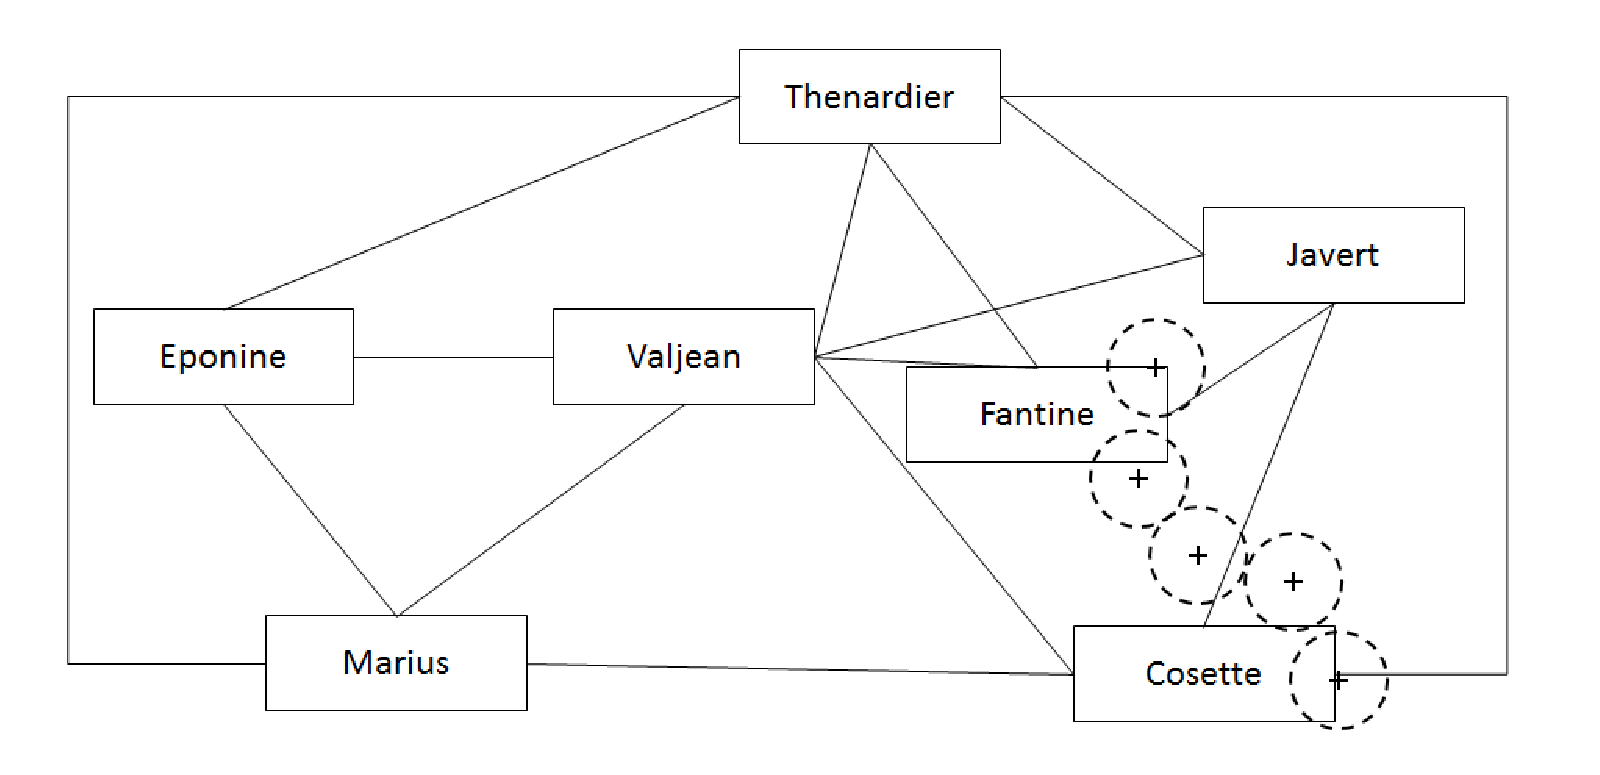
\includegraphics[width=0.99\linewidth]{images/MiserablesSimple.eps}
  \caption{: A network diagram with major characters of Les Miserables. The dashed circles represent a user's gazes. Here, most gaze points are adjacent to Fantine and Cosette. }
    \label{fig:MiserablesSimple}
\end{figure}

Moreover, the visual objects are shown in the Les Miserables visualization stand for actual data: the characters in the novel. So, mapping gazes to the visual objects let us in turn map the user's interest to data elements, such as Fantine and Cosette. Moreover, by looking at the properties of the data that users are viewing, we can relate visual interest to semantic data subsets or perspectives. For example, Fantine and Cosette are both female characters and, based solely on the few gaze samples depicted in our example. We could conclude that the user is viewing female characters. In other words, we can track the user's interest in data subsets defined based on gender. Similar data subsets could be identified based on central or secondary characters, positive or negative characters, etc. We call this eye-tracking data analysis in ``data space'' or data of interest (DOI) analysis.

We hypothesize that this is a compelling alternative to traditional analysis methods, primarily AOI (area of interest) analyses. Using conventional AOI-based approaches, analyzers would be required to define AOIs over already rendered 2D stimuli. In our example, and most real-life visualizations, this would be time-consuming because of the many visual objects displayed on the screen. Moreover, the 2D layout of the visualization may change in response to user interactions (e.g., users move node), in which case the AOI annotations would need to change. Moreover, AOIs are not annotated by any attributes so defining AOIs on characters wouldn't implicitly mean that we could also track other data subsets such as based on gender.  

However, as described in Chapter~\ref{chap:Intro}, mapping gazes to individual data objects is bound to be imprecise since eye-trackers produce noisy, low-resolution data. Figure ~\ref{fig:MiserablesGaze} illustrates this. We can use the na\"{i}ve approach of mapping gazes to the nearest visual object. Using this approach, we can confidently map $g_1, g_2$ to Fontaine, and $g_4, g5$ to Cosette. However, it's less clear what we should do about $g_3$ since it's squarely between the two nodes. 

\begin{figure}[htb]
  \centering
  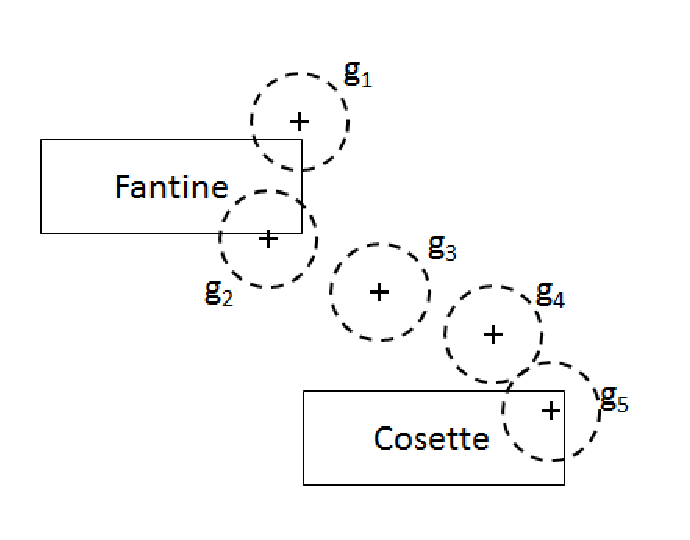
\includegraphics[width=0.5\linewidth]{images/MiserablesGaze.eps}
  \caption{: Using proximity alone to map gazes to visual objects. We have 2 rectangles Fontaine and Cosette, and five gazes $g_1, g_2, g_3, g_4, g_5$. Each gaze is to be mapped to either Fontaine or Cosette. $g_1, g_2$ maps to Fontaine and $g_4$ map to Cosette. However, $g_3$ cannot be mapped directly to neither Fontaine nor Cosette. }
    \label{fig:MiserablesGaze}
\end{figure}
\section{Methods}
\label{sec:DOICollectionMethods}
Initially, we assume that our eye-tracking experiments will use visualizations which are accessible for instrumentation to programmers. Thus, graphical information (e.g. position, size, shape) of internal visualization primitives (e.g. circles representing nodes in a graph) are available at rendering time. 

Our proposed methods will only operate over visualizations with open source code. Such scenario is a limitation of our work. However, we claim that open source code libraries are gaining popularity over proprietary applications. Figure~\ref{fig:WebUsageChart} shows a comparison between two popular visualization libraries: d3JS (open source code) and FusionChart (proprietary application).

\begin{figure}[htb]
  \centering
  \includegraphics[width=0.99\linewidth]{images/WebUsageChart.eps}
  \caption{: Comparison of number websites using d3js and FusionChart in their homepages. Data collected from http://trends.builtwith.com/. }
	\label{fig:WebUsageChart}
\end{figure}

We aim to map gazes to visualization primitives using our viewed-object-detection algorithm. Our algorithm will seek to compute ``object viewing scores'' that express the likelihood that an object is perceived given a particular gaze sample. The viewed-object-detection algorithm outputs object viewing scores from which we can construct DOI data. We aim to develop viewed-object-detection algorithm incrementally in three stages. First, we plan to detect objects using the na\"{i}ve approach of AOI binning. We will consider each visual object as an AOI. In this method, we consider the objects as `viewed' where most recent gaze points land. Second, we intend to develop a method for calculating a probabilistic fuzzy score for each object based on the proximity of gaze landing to the object. Third, we plan to build on Salvucci's method~\cite{Sal00} to develop an algorithm to calculate the object viewing score based on the probabilistic score and an additional prediction score. The prediction score will be calculated based on the semantic content of the data. 

\begin{figure}[htb]
  \centering
  \includegraphics[width=0.99\linewidth]{images/System.eps}
  \caption{: Detection of viewed objects in generative visualizations.}
	\label{fig:System}
\end{figure}

We depict our general approach for collecting DOI data in Figure~\ref{fig:System}. Eye-trackers supply gaze samples in screen space. The `Screen to Model Transformation' module (Figure~\ref{fig:System}) will transform these gaze samples to the visualization model space. The `Renderer' module will render the visualization, and supply information regarding shapes and positions of visual objects, and model transform information. Afterward, our algorithm will combine gaze samples and visual object positions to detect viewed objects by calculating object-viewing-scores. A prediction module will use information about what a user has seen in the past and interacted with, to infer what objects the user is likely to be viewing presently. In Figure~\ref{fig:System}, we observe that the eye-tracker and the visualization model pass the gaze positions and visualization information respectively to the viewed object detection module. We hypothesize that this will reduce the inaccuracies previously illustrated, by allowing us to discriminate which visual object is users is likely to be looking at when gazes land near multiple objects.
We provide more details about the three stages of developing viewed-object-detection algorithm below. 

\subsection{AOI-Based Viewed Object Detection}
\label{sec:AOIBasedViewedObjectDetection}

A na\"{\i}ve approach is to treat object shapes as dynamic AOIs and determine that a viewed object is that with the most recent fixation landing in its AOI. Analysts use manually drawn AOIs are in the same manner in offline eye-tracking data analysis, and the similar concept of objects of interest (OOIs) has been proposed already by Stellmach et al.~\cite{Ste10} for generative 3D content.

The problem with this approach is that for highly granular visual content, such as individual nodes or labels, users often fixate in the vicinity of the object rather than on the object itself. A potential solution is to pad object AOIs to be slightly larger than the objects. However, larger AOIs may lead to overlaps in cluttered visualizations. We demonstrate and quantify these observations in Section~\ref{sec:DOICollectionEvaluation}. Ultimately, the problem lies with an inability to determine with absolute certainty what a user is observing. We describe it in more detail in the next section.

\subsection{A Probabilistic Approach to Viewed Object Detection}
\label{sec:ProbabilisticObjectDetection}

Unlike mouse input, eye-tracking can only indicate a small screen region that a user is fixating, rather than a particular pixel. Typically, such regions are about one inch in diameter, though specific values depend on viewing conditions. As such, it is impossible to tell with certainty which objects a user is viewing, if the user is fixating in the vicinity of multiple close objects (Figure~\ref{fig:discreminateFig4}(a)). Such situation is not a significant problem for traditional AOI analyses, which use large AOIs. Conversely, we aim to detect the viewing of granular visual content, such as network nodes or glyphs, in cluttered visualizations.

\begin{figure}[htb]
  \centering
  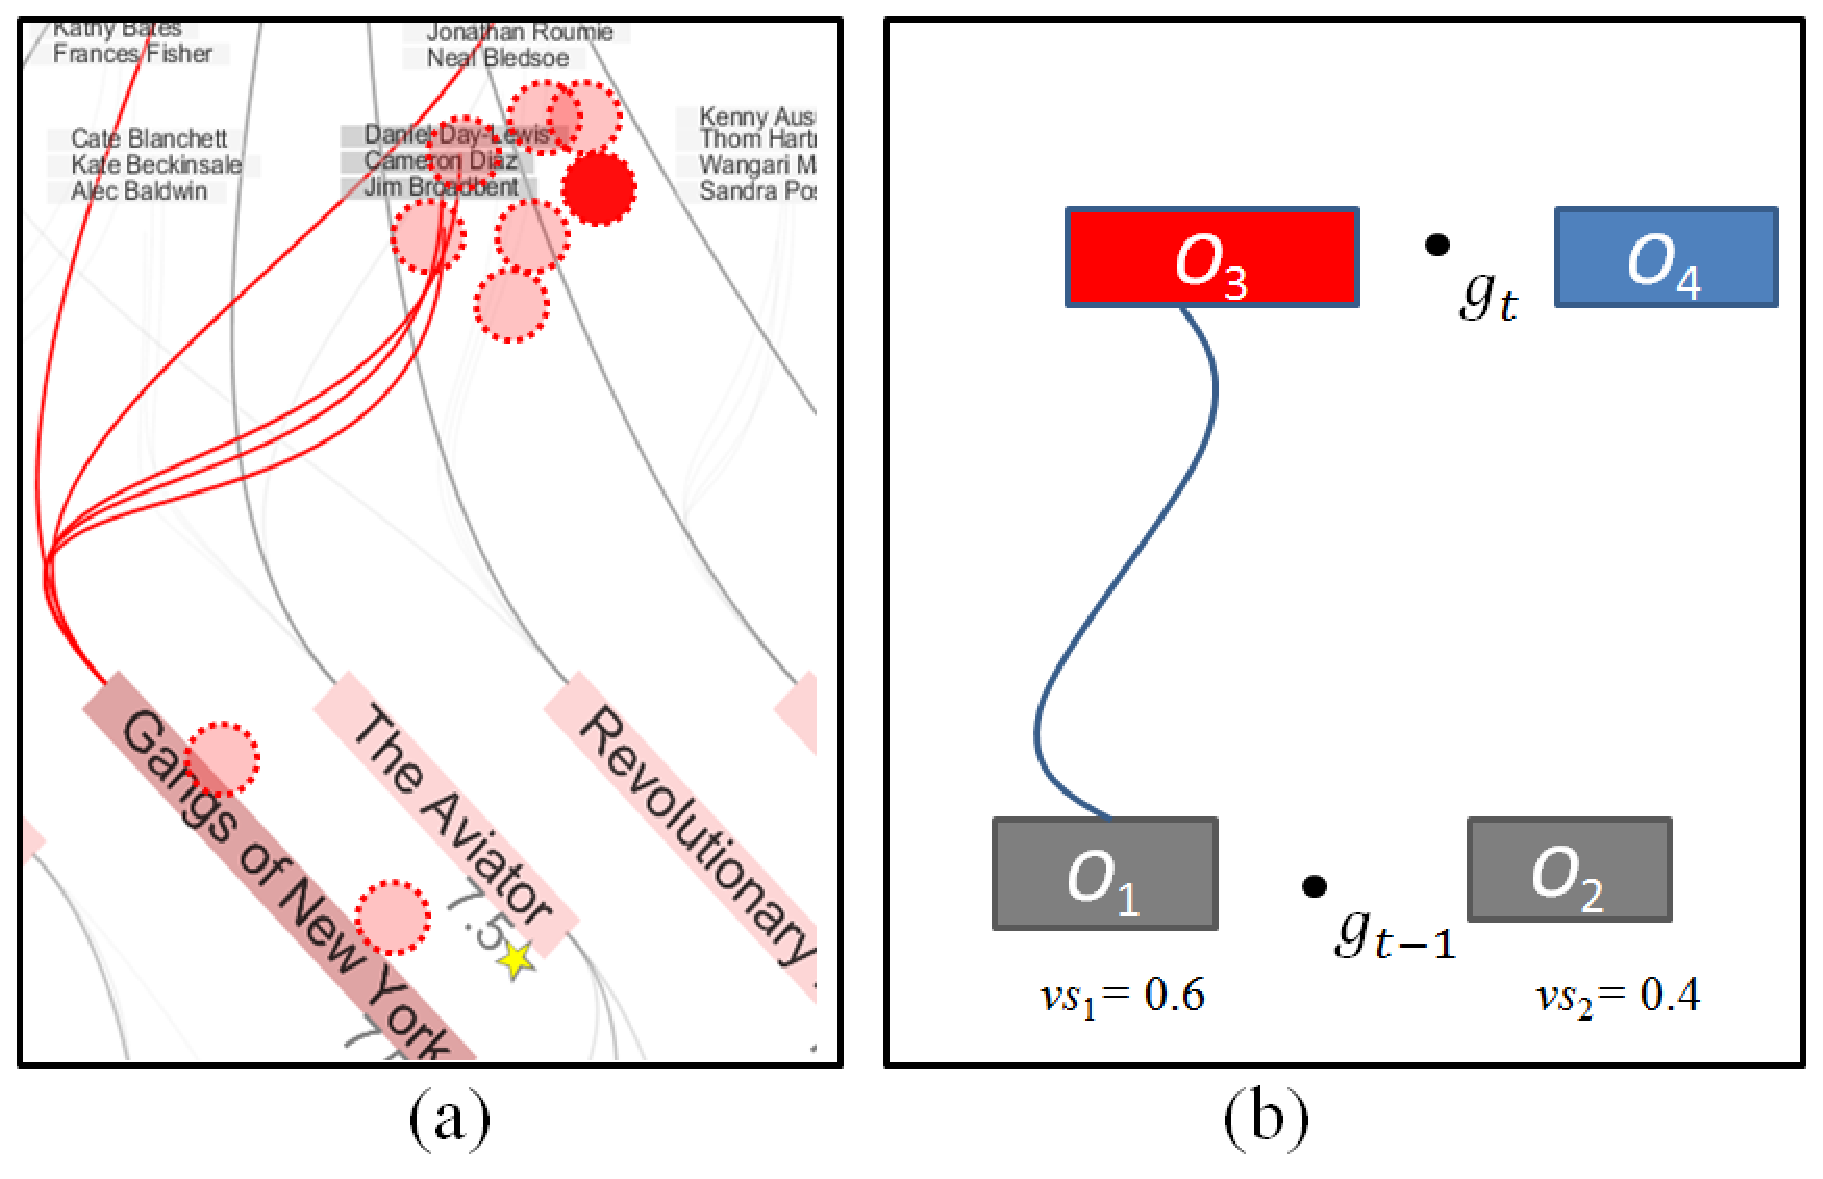
\includegraphics[width=\linewidth]{images/discreminateFig4.eps}
  \caption{(a) A real visualization example in which a user fixates in the vicinity of multiple close object groups (red dot). (b) predictive method: even though the latest gaze sample falls equidistantly between visual objects $O_3$ and $O_4$, we suspect that $O_3$ is the more likely viewing target given that it is highlighted and connected to $O_1$, which is likely to have been the object that the user viewed previously ($vs_1=0.6 > vs_2 = 0.4$). }
	\label{fig:discreminateFig4}
\end{figure}

We advocate for a fuzzy interpretation of gaze data and detect likelihoods that objects are viewed rather than certainties. To this end, we can compute object gaze scores $gs$ (for all objects $i$ in a visualization, and at all times $t$). The gaze scores range between zero- user did not view the object, and one-user certainly viewed the object. We show them in Figure~\ref{fig:gazeScoreFig3} and Formula~\ref{eq:GS}. 

\begin{figure}[htb]
  \centering
  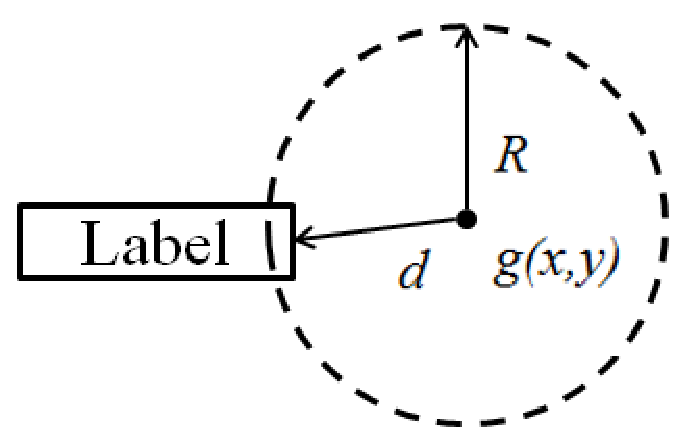
\includegraphics[width=0.4\linewidth]{images/gazeScoreFig3.eps}
  \caption{Calculating gaze score $gs$ for a gaze sample landing near an object. $d$ is the distance from the object to the gaze sample, and $R$ approximates the size of the user's foveated region.}
	\label{fig:gazeScoreFig3}
\end{figure}

%Formula 1
\begin{equation}
gs_{i,t} = 1 - \min (1, (\frac{d}{R}))
\label{eq:GS}
\end{equation}

The region of radius $R$ used in the formula is analog to the user's foveated region, and as such needs to be constant in screen space. Thus, if we zoom the view in or out, $R$ needs to be scaled accordingly in model space to remain constant in screen space.  Salvucci et al.~\cite{Sal00} and Okoe et al.~\cite{Okoe14} used similar approaches.

Finally, we note that the object scores ($gs$) do not directly equate to probabilities. The distinction is important because our implementation can detect two objects as being viewed simultaneously ($gs_1 = 1$ and $gs_2=1$). We think this is appropriate since a person can in fact visually parse multiple objects at the same time if they fall within the user's foveated region, and even think of multiple objects as a unit for specific task purposes.



\subsection{A Predictive Algorithm for Viewed Object Detection}
\label{sec:MehthodsIntelligentAlgorithm}

Salvucci and Anderson described the concept of ``intelligent gaze interpretation'' in the context of a gaze-activated interface ~\cite{Sal00}. They more accurately detected which interface control a user was gazing at, by integrating both the proximity of the gaze to the control, and the likelihood that the control was the target of a gaze-interaction, based on the current state and context of the interface. Formally, their algorithm identified the most likely currently viewed item $i_{viewed}$ by solving Equation~\ref{eq:IViewed}.

\begin{equation}
i_{viewed} = \displaystyle \argmax_{i\in I}%[Pr(g|i)\cdot Pr(i)]
\label{eq:IViewed}
\end{equation}

In Equation~\ref{eq:IViewed}, $Pr(g|i)$ is the probability of producing a gaze at location $g$ given the intention of viewing item $i$, and $Pr(i)$ is the prior probability of an item $i$  being the target of a gaze interaction. Salvucci and Anderson based these prior probabilities on assumptions about how we may use an interface, and hard code them into their system.  

We adapt Salvucci and Anderson's paradigm to solve the ambiguous case when a gaze sample lands close to multiple objects (e.g.,  Figure~\ref{fig:discreminateFig4}(a)). For example, in a network visualization, we may assume that a user who has just viewed a node $n$, will more likely view one of $n$'s neighbors than another random node, perhaps especially if the user previously highlighted node $n$ and its outgoing edges.  In Section~\ref{sec:DOICollectionEvaluation} we show quantitatively that this assumption holds for one tested visualization.  

We consider the simplified scenario in Figure~\ref{fig:discreminateFig4}(b): four visual objects ($O_{1\ldots 4}$), two of which are connected ($O_1$ and $O_3$), and one of which is highlighted ($O_3$), are shown on the screen. A new gaze sample registers between $O_3$ and $O_4$ at time $t$. Intuitively, it is more likely that the user viewed $O_3$ since it is highlighted. Moreover, if we knew that $O_1$ was seen just before the current moment and assume that users view neighboring nodes together, then this likelihood becomes stronger.         
 
Formally, we compute $vs_{i,t}$  (i.e., the viewing score $vs$ of object $i$ at time $t$) by weighing the gaze score $gs_{i,t}$ described in Section~\ref{sec:ProbabilisticObjectDetection} by a prediction score $ps_{i,t}$ that object $i$ is a viewing target at time $t$:  
%Formula 2
\begin{equation}
vs_{i,t} = gs_{i,t} \times ps_{i,t}
\label{eq:VS}
\end{equation}

This prediction score is computed based on the likelihood that an object is viewed if another object (e.g.,  a node's neighbor) was seen just before it. Specifically, $ps$ is derived from a viewing transition function $T$ between objects:  $T(j,i)$ gives the likelihood that object $i$ is viewed after object $j$ is perceived. We will assume that $T(j, i)$ is input to our algorithm. Concrete examples of what $T(j, i)$ could be linked to are whether objects $i$ and $j$ are somehow connected or related, or whether they are part of a special group (e.g., highlighted elements). Moreover, connections could be either visual, such as an explicit edge or leader line or an implicit sharing of similar visual attributes (e.g., color, shape), or semantic (e.g., both nodes are actors). More examples of $T(j, i)$ functions, and means of defining them are described throughout this chapter.

To compute $ps$, we could consider $ps_{i,t} = T(j,i)$ but that would involve knowing $j$, the previously viewed object, with absolute certainty. As exemplified in Figure~\ref{fig:discreminateFig4}(b), we often cannot unequivocally determine which item was viewed at a given time: $O_1$'s previous viewing score ($vs_{1,t-1}=0.6$), is just slightly larger than $O_2$'s viewing score ($vs_{2,t-1}=0.4$), and thus an absolute choice of $O_1$ over $O_2$ as previously viewed element would be rather arbitrary.  In other words, we cannot say with absolute certainty which of the two objects was viewed before because the user fixated between them. 

In more general terms, our computation of $ps_{i,t}$ must account for multiple items $j$ that may have been viewed before. These items $j$ are those with a previous visual score $vs_{j,t-1}$ that is greater than $0$.  As such, we compute $ps_{i,t}$ as a weighted average of all transition probabilities from objects $j$ with $vs_{j,t-1} > 0$ , to our current item $i$. The weights are given by the likelihood that an object $j$ was viewed before - in other words by its previous viewing score $vs_{j,t-1}$. This computation is captured by Formula~\ref{eq:ps}.  

%Formula 4
\begin{equation}
ps_{i,t} = \frac{\displaystyle\sum_{j} {vs_{j,t-1} \times T(j,i)}}{\displaystyle\sum_{j} vs_{j,t-1}} \text{ , where  } \parbox{15em}{$0\leq i \leq n$ and $gs_{i,t} > 0$\\$0\leq j \leq n$ and $vs_{j,t-1} > 0 $\\ $0\leq j \leq n$ and $gs_{j,t} = 0$ }
\label{eq:ps}
\end{equation} 

Finally, Formula~\ref{eq:ps} needs to add a significant constraint. Intuitively, our approach means that previously viewed objects $j$ act as referees with varying degrees of influence (i.e., previous visual scores) in a competition between currently viewed items $i$. This analogy provides the intuition for the important constraint: an object should not referee a competition that it is part of. For example, in our simplified scenario, using $O_3$ as a previous element in a competition between itself and $O_4$ would result in an open feedback loop and should be avoided. Formula~\ref{eq:ps} reflects this restriction by the 3rd inequality.  We provide the algorithm pseudocode below.

\begin{algorithm}
\caption{Viewed Object Detection Algorithm}
\label{alg:ObjectDetection}
\begin{algorithmic}[1]
\State \textbf{Inputs: } 
\Statex $O_{i, \ldots, n}$= tracked visualization objects (shapes, positions)
\Statex $g(x,y) = $ gaze sample in model space (time $t$)
\Statex $T(i,j) = $ viewing transition function ($T(i,j) \in [0,1]$)
\State \textbf{Outputs:}
\Statex $vs_{i,t} = $ momentary viewing scores of all objects ($i = 1, \ldots, n$). 
\For{$i \gets 1 \text{ to } n$}
	\State Compute $gs_{i,t}$	using Formula~\ref{eq:GS}
\EndFor
\State $max \gets 0$
\For{$i \gets 1 \text{ to } n$}
	\If{$gs_{i,t} > 0$} \label{algLine:PredictionScoreLines}
		\State Compute $ps'_{i,t}$	using Formula~\ref{eq:ps}
		\If{$ps'_{i,t} > max$}
			\State $max \gets ps'_{i,t}$
		\EndIf
	\EndIf
\EndFor
\For{$i \gets 1 \text{ to } n$}
	\State $vs_{i,t} \gets gs_{i,t} \times \frac{ps'_{i,t}}{max} $
\EndFor
\end{algorithmic}
\end{algorithm}

Last, we note that to optimize for speed, we only compute prediction scores for objects with non-zero gazes (Algorithm~\ref{alg:ObjectDetection}, line~\ref{algLine:PredictionScoreLines}). Also, we compute viewing scores for every gaze sample, rather than every fixation. We believe that doing so leads to results that are less dependent on how fixations are computed and more robust. Since our eye tracker's sampling rate is $120$Hz, the scores $vs_{j, t-1}$ were calculated just $8$ms ago, an interval shorter than the time it takes for people to shift their attention to a new object. As such, instead of using the raw $vs_{j,t-1}$ score, we use an average of the last several viewing scores. Moreover, for all practical purposes, the term $vs_{j,t-1}$ should be replaced in the previous formulas by $ \sum_{k=1}^{k=15}{vs_{j,t-1}}$. Given, our eye tracker's $120$Hz temporal resolution, it produces gaze samples in approximately $125$ms. Thus, such time window we observed to be close to an average fixation duration. However, we note that our algorithm can take as input fixations rather than individual gaze samples, in which case this step would not be necessary. Moreover, additional smoothing and filtering such as those summarized by Kumar et al.~\cite{Kum08} could be used to clean gazes before feeding them into our algorithm. We tried removing gaze samples with high velocity as they are likely to be part of saccades but observed no discernable improvement in our algorithm's output. 


{\bf Performance analysis:} The algorithm traverse through all objects ($n$) to find those in the proximity of a gaze sample or fixation ($k_t$). Then, to compute $ps$ for each of the $k_t$ potentially viewed elements, the algorithm iterates over $k_{t-1}$ objects with non-zero viewing scores from the previous iteration. The algorithm is linear if we consider the number of objects that a user can view at any time to be a constant. Such case is not true for example if the visualization is zoomed out too much and falls entirely within the algorithm's $R$ radius. However, in such cases, the output of the algorithm would be meaningless, and we should abort the algorithm.
\section{Evaluations}
\label{sec:DOICollectionEvaluation}

\subsection{Overview}
We instrumented D{\"o}rk's interactive PivotPaths visualization of multifaceted data~\cite{Dor12}. Figure~\ref{fig:pivotpaths} shows the visualization which links to the popular internet movie database (IMDB). We collected data from $9$ subjects, each using our instrumented visualization for $50$ minutes on a series of structured and unstructured tasks. We used this data to test the validity and effectiveness of our approach in two ways. 

First, we compared the output of the predictive algorithm to human annotations. We found that data collected automatically was on average as similar to human annotations, as human annotations were analogous to each other. We conducted this analysis for all three viewed detection algorithms described in Sections~\ref{sec:AOIBasedViewedObjectDetection} to~\ref{sec:MehthodsIntelligentAlgorithm} and found that the AOI algorithm performs poorly compared to the other two and that the predictive algorithm improves detection accuracy by about $5\%$  (Figure~\ref{fig:quantitative}). 

Second, we showed that our instrumentation method provides relevant information that we can leverage in novel ways. We showed both qualitatively and quantitatively that viewed objects detected automatically were closely correlated to tasks people were asked to do, and that data collected automatically from many users could answer novel questions about how people use visualizations (Figures~\ref{fig:heatmap}~and~\ref{fig:RelevanceDiagram}). We also demonstrated quantitatively that the viewing-biases our predictive algorithm exploits exist and are significant: our users were much more likely to look at objects that were highlighted and connected to each other (Table~\ref{tab:TransitionFromMovie},~\ref{tab:TransitionFromActor},~\ref{tab:TransitionFromDirector}, and~\ref{tab:TransitionFromGenre}).  Each table shows data for a movie element (e.g. movie, actor, director) to a target object divided by: (i) type of source and target; (ii) whether the target was highlighted (H); (iii) whether the target was highlighted and connected to the source (HC); (iv) and whether source and target were neither highlighted nor connected. Columns show: (i) the number of direct transitions for the source/target combination; (ii) the observed transition probability from the source to that target; (iii) the (unbiased) probability of transition between source and target if all elements had equal probability to be viewed; (iv) the ratio between observed and unbiased transition probabilities.


\subsection{Instrumenting a Sample Visualization}
\label{sec:InstrumentingVisualization}

\begin{figure}[htb]
  \centering
  \includegraphics[width=\linewidth]{images/PivotPath.eps}
  \caption{PivotPaths visualization of IMDB data. Movies are displayed in the center of the screen, actors at the top, and directors and genres share the bottom space. Actors, directors, and genres associated to movies are connected through curves. Users can highlight objects and their connected neighbors by hovering over them.}
	\label{fig:pivotpaths}
\end{figure}
Our PivotPaths visualization of IMDB data renders movies in the center of the screen, actors on top, and genres and directors at the bottom (Figure~\ref{fig:pivotpaths}). The visualization connects actors, directors, and genres by curves to the associated movies. Moreover, the elements are larger, and their connections more salient, if they associate with multiple movies. Actors, genres, and directors are colored distinctively, which is particularly important for genres and directors since they occupy the same visual space. Such views are created in response to users' searches for specific movies, actors, and directors, and show only data that is most relevant to the search. As shown in Figure~\ref{fig:pivotpaths}, users can hover over visual elements to highlight them and their connections. Users can also click on visual elements to transition the view to one centered on the select element. Finally, users can freely zoom and pan. 

We opted to instrument this visualization for three reasons. First, it is highly interactive and would be significantly difficult to analyze using traditional analyses. Second, it contains visual metaphors, graphic primitives, and interactions typical of a wide range of visualizations. Third, movie data is familiar to a wide variety of users.  

To choose transitions functions $T$ underlying our predictive algorithm, we made simple assumptions about how the visualization is used, an approach also employed by Salvucci~\cite{Sal00}. We assumed that transitions between connected items would occur more often than between unconnected objects. We also assumed that highlighted elements are more likely to be viewed than those that are not. We translated these assumptions into specific weights, as exemplified in Table~\ref{tab:Transition2}. We show in Section~\ref{sec:EvalResults} that these assumptions hold for the instrumented visualization and the subjects that used it in our study. 

\begin{table}[htbp]
\caption{Example transition probabilities in our instrumented visualization (assumed).}
	\centering
		\begin{tabular}{|l|c|}
			\hline
			 \multicolumn{2}{|c|}{Assumed visual and transition weights} \\ \hline
			Movie to unconnected actor & 1\\\hline
			Movie to connected actor & 3\\\hline
			Movie to unconnected genre & 1\\\hline
			Movie to connected genre & 3\\\hline
			Movie to unconnected director & 1\\\hline
			Movie to connected director & 3\\\hline			
		\end{tabular}
	
	\label{tab:Transition2}
\end{table}

Finally, as part of the instrumentation, our system collected screen shots, interactive events (e.g., zooming, panning), raw gaze samples captured at a rate of $120$Hz, and visual elements that users viewed. For each viewed element we recorded the type (i.e., movie, actor, director, genre), its label, its gaze score ($gs$), its prediction score ($ps$), and the aggregated viewing score ($vs$). All recorded data was time stamped.

\subsection{Study Design}
\label{sec:EvalStudyDesign}

\noindent\textbf{Setup: } We used the IMDB visualization described above, and an SMI RED-120Hz connected to a 17'' monitor. Subjects were seated approximately $30''$ away from the display. 

\noindent\textbf{Subjects:} We collected data from $9$ graduate and undergraduate students aged between $20$ and $30$ years. Six subjects were male, and three were female. All were paid $\$10$ for their participation. 

\noindent\textbf{Protocol:} At first, we gave the subjects a description of the study's purpose and protocol. Next, we introduced them to the visualization and asked to perform a few training tasks. This introductory part lasted on average $10$ minutes. The main section of the study followed, involved multiple instances of four types of tasks, and lasted approximately $50$ minutes. 

\noindent\textbf{Tasks:} Subjects completed four types of structured and unstructured tasks. To solve structured tasks, subjects had to consider data that was better defined and less variable than in unstructured tasks. This made it easier for us to test the degree to which object-detection was aligned with the task associated data. On the other hand, data collected in unstructured tasks may be more ecologically valid. We limited the time we allowed subjects to spend on each task for two reasons: to manage the total duration of the study and to make results comparable across users.

\begin{itemize}
\item \textbf{Task1 (structured):} Finding four commonalities between pairs of movies. The tasks were limited at three minutes each, and subjects solved the following four instances of this task: (a) Goodfellas and Raging Bull; (b) Raiders of the Lost Ark and Indiana Jones and the Last Crusade; (c) Invictus and Million Dollar Baby; (d) Inception and The Dark Knight Rises.  
\item \textbf{Task2 (structured):} Ranking collaborations between a director and three actors ($2$ minutes, $4$ instances): (a) Ang Lee; (b) Tim Burton; (c) James Cameron; (d) David Fincher.  
\item \textbf{Task3 (semi-structured):} Given three movies, subjects were asked to recommend a fourth ($5$ minutes, $3$ instances): (a) Catch Me If You Can, E.T. the Extra-Terrestrial, and Captain Phillips; (b) To Kill a Mockingbird, The Big Country, and Ben-Hur; (c) Inglourious Basterds, The Avengers, and Django Unchained.

\item \textbf{Task4 (unstructured):} Given a brief and incomplete description of the ``Brat Pack'', a group of young actors popular in the 80's, subjects were asked to find additional members and movies they acted in. Subjects solved one such task, in approximately $5$ minutes. 
\end{itemize}


\subsection{Results}
\subsubsection{Data Collected Automatically is Similar to that of Human Annotators}
\label{sec:EvalResults}

We tested whether the outputs of the three algorithms described in Sections~\ref{sec:AOIBasedViewedObjectDetection} to~\ref{sec:MehthodsIntelligentAlgorithm} (AOI, probabilistic, and predictive) are comparable to annotation data obtained from human coders who inspected screen-captures with overlaid gaze samples and manually recorded what subjects viewed. We included in our analysis the AOI algorithm version which uses padded AOIs (Section ~\ref{sec:AOIBasedViewedObjectDetection}). As shown in Figure~\ref{fig:quantitative}, we found that the overlap between human annotations and the predictive algorithm's output is similar to the overlap within the set of human annotations and that the predictive algorithm outperforms the others. 

We enlisted the help of five coders and asked them to annotate eye-tracking data corresponding to one task of approximately three minutes, for each of six subjects.  The task was the same for all coders - task 1b. The six subjects were selected randomly and were the same for all five coders. Coders spend approximately one hour per subject completing their annotation. This long duration meant it was unfeasible to code data from more users or more tasks. Four coders completed all six assigned annotation tasks, while one was able to annotate the data of only three subjects. 

Coders used an application that allowed them to browse through screen captures of a users' activity with overlaid gaze coordinates. We asked coders to advance through the videos in $100$ms time-steps, determine what visual objects their assigned subjects were viewing, and record those objects along with the start time and the end time of their viewing. If unsure which of multiple viewed objects, coders were allowed to record all of them.  

We transformed each coder's annotation into temporal vectors with $100$ms resolution. These vectors contained at each position one or several objects that were likely viewed by the subject during each $100$ms time-step. We then created similar representations from our automatically collected data. Finally, we defined a similarity measure between two such vectors as the percentage of temporally aligned cells from each vector that were equal. We defined equality between vector cells as a non-empty intersection between their contents.  

For each algorithm, we computed the similarity of its output for each subject's data to all available human annotations of the same data.  This yielded $4$ coders $\times$ $6$ subjects $+$  $1$ coder $\times$ $3$ subject $=$ $27$ similarities per algorithm. We averaged these similarities and plotted them as the first four bars in Figure~\ref{fig:quantitative}. Then, we compared each coder's annotation of a subject's data to all other available annotations of the same data. Since we had five annotations for three subjects, yielding $3$ subjects $\times$ $10$ annotation pairs $=$ $30$ similarities. Moreover, four annotations for the remaining subjects, yielding $3$ subjects $\times$ $6$ annotation pairs $=$ $18$ similarities. Finally,  we obtained $48$ similarities, which we averaged and plotted as the last bar of Figure~\ref{fig:quantitative}. The first four bars show the overlap between the outputs of
the three algorithms described in Section~\ref{sec:DOICollectionMethods} (padded-AOI approach included), and annotation results of human coders. The last bar shows the overlap within the set of human annotations. Values correspond to averages over multiple tasks, multiple subject data sets, and multiple annotators, and are computed as described in Section~\ref{sec:EvalResults}. Error bars extend by one standard error.

Our collected data allowed us to perform this analysis for all three algorithms described in Section~\ref{sec:DOICollectionMethods}, as well as for the padded version of the AOI method. If we only consider gaze scores $gs$ that are equal to one (Section~\ref{sec:AOIBasedViewedObjectDetection}) and no predictive component, we essentially have the output of the AOI algorithm. If we limit the analysis to $gs$ scores alone, without the prediction component described in Section~\ref{sec:MehthodsIntelligentAlgorithm}, we have the output of the probabilistic approach described in Section~\ref{sec:ProbabilisticObjectDetection}.

\begin{figure}[htb]
  \centering
  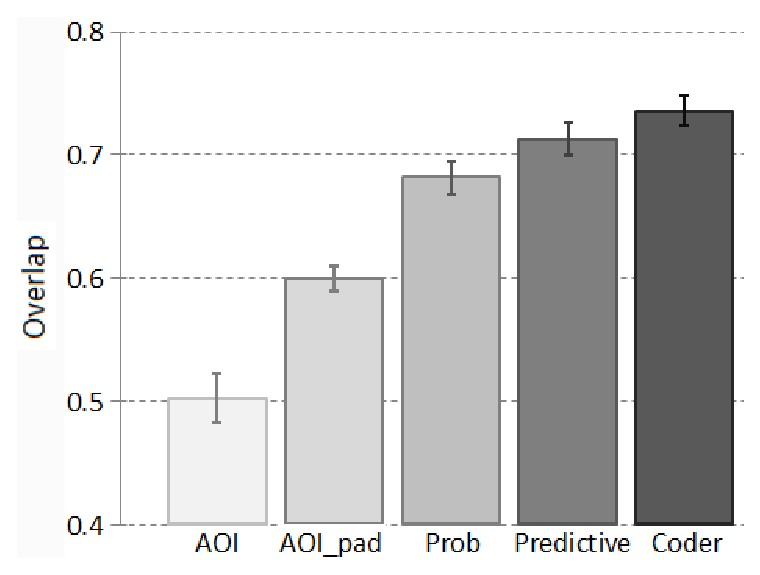
\includegraphics[width=0.6\linewidth]{images/algosComparison.eps}
  \caption{Comparison between automated and manual viewed object detection. }
	\label{fig:quantitative}
\end{figure}


\subsubsection{Data Collected Automatically is Relevant and Useful}
\label{sec:EvalDataCollected}

We used two analyses to show that data collected automatically is tightly correlated with the tasks that users had to do. We chose this evaluation for two reasons. First, it provides evidence that our instrumentation approach can be used to solve the inverse problem: an observer or analyst who is unfamiliar with a subject's intentions can determine what these are by looking at the subject's visual interest data. 

Second, it demonstrates how the automated collection of eye-tracking data can facilitate novel insights into how we use visualizations. Our approach allowed us to quantify that a users' interest in a visual item present on the screen decays exponentially with a decrease in the items' relevance to a task. It is a well-known fact in visualization community that users follow ``information scent'' when solving tasks visually~\cite{informationscent2003}. Thus, from this fact, we were able to quantify this effect. 
 
\vspace{2mm}\noindent
\textbf{First }, we created heatmap representations from our collected data (Figure~\ref{fig:heatmap}) to illustrate qualitatively the strong connection between the tasks our subjects performed and the data we collected. We listed viewed objects vertically, discretized viewing scores by averaging them over $500ms$ intervals, and arranged them horizontally. Thus, time is shown horizontally, viewed objects vertically, and intensity of heatmap cells indicate the degree to which an object was viewed at a given time. The viewed objects listed vertically were colored based on their type (movie, actor, director, genre) and could be sorted by either first time they were viewed, the amount of viewing activity, or type.

Figure~\ref{fig:heatmap} shows the data collected from a subject performing Task 1b: finding commonalities between two Indiana Jones movies. Horizontal cells, shown horizontally, represent user eye activity in 500ms time increments. Viewed objects are viewed vertically; cell darkness indicates viewing intensity (black: high; white: low); viewed items are ordered by category (genre, director, movie, actor). We notice that elements viewed often are tightly connected to the subjects'  task.   Moreover, we can distinguish a temporal pattern: the movies featured in the task description were viewed throughout the analysis, actors were considered early on, followed by genres, then directors, and ultimately a quick scan of other movies. We observed this pattern for most subjects and thought it was caused by the ordering used in the task's phrasing: we asked subjects to determine actors, genres, and directors that were common between the two movies.   

\begin{figure}[!ht]
  \centering
  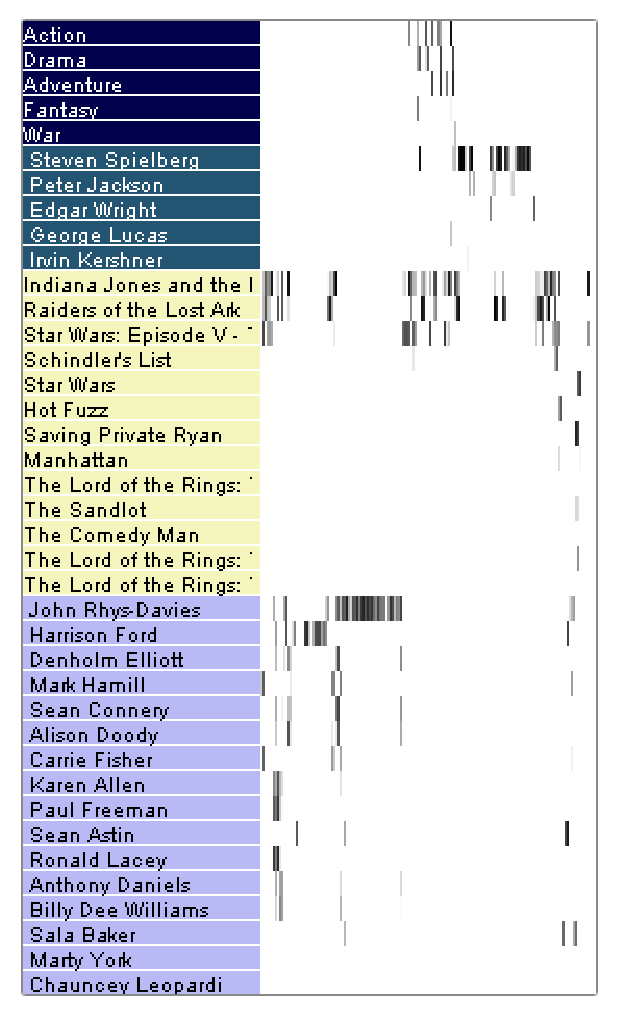
\includegraphics[width=0.75\linewidth]{images/heatmaps.eps}
  \caption{Heatmap views of one subject's activity on Task 1b.}
	\label{fig:heatmap}
\end{figure}

\vspace{2mm}\noindent
\textbf{Second}, we formalized the relevance of each visual item to a particular task and plotted this relevance against the amount of interest that each item attracted (Figure~\ref{fig:RelevanceDiagram}). In Figure~\ref{fig:RelevanceDiagram}, each task is plotted in its type's corresponding chart as a subdivision across multiple relevance categories. Relevance was computed as described in Section~\ref{sec:EvalDataCollected}, and plotted for all objects that were visible to subjects during each task. The average interest in objects with the same task relevance are linked by separate polylines for each task; errors bars extend from the averages by one standard error. These plots quantify the degree to which tasks determine users' interest in visual objects and demonstrate that our instrumentation captures relevant data.    

We formalized the relevance of a visual item to a task as $\text{Relevance}~=~1/(1+d)$, where $d$  is the shortest graph distance between that item and items mentioned directly in the task description.  To exemplify, the relevance of Goodfellas and Ranging Bull to task 1a is $1$ as they are the focus of the task, that of Martin Scorsese is $1/2$  because he directed both movies, while that of other movies directed by Scorsese is $1/3$. This definition is not entirely accurate as items might be relevant to a task even though we did not directly mention them in the description.  For instance, items that eventually constitute a user's answer will elicit more attention. 

Figure~\ref{fig:RelevanceDiagram} facilitates several insights. First, even though many items were shown to subjects during their tasks, only very few were viewed for significant periods of time, and many were not viewed at all. Second, the types of user-focused data, correlate with the particularities of each task. For example, Task 3 involved movie recommendations and Figure~\ref{fig:RelevanceDiagram} illustrates that genres and directors were viewed significantly more than in task 4, which involved determining the identity of a group of actors and seemed to drive users' attention towards actors. 

\begin{figure}[!htb]
  \centering
	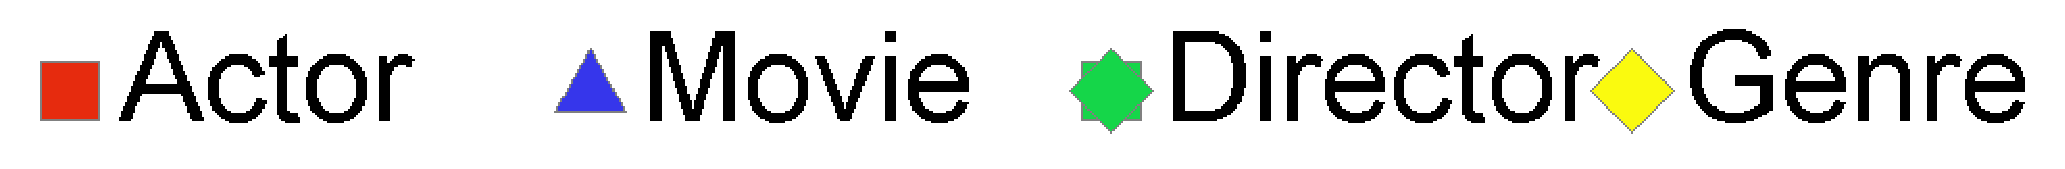
\includegraphics[width=0.45\linewidth]{images/Legends.eps}
  \includegraphics[width=0.6\linewidth]{images/RelevanceDiagramTask1.eps}
	
	\includegraphics[width=0.6\linewidth]{images/RelevanceDiagramTask2.eps}
	
	\includegraphics[width=0.6\linewidth]{images/RelevanceDiagramTask3.eps}
	
	\includegraphics[width=0.6\linewidth]{images/RelevanceDiagramTask4.eps}
	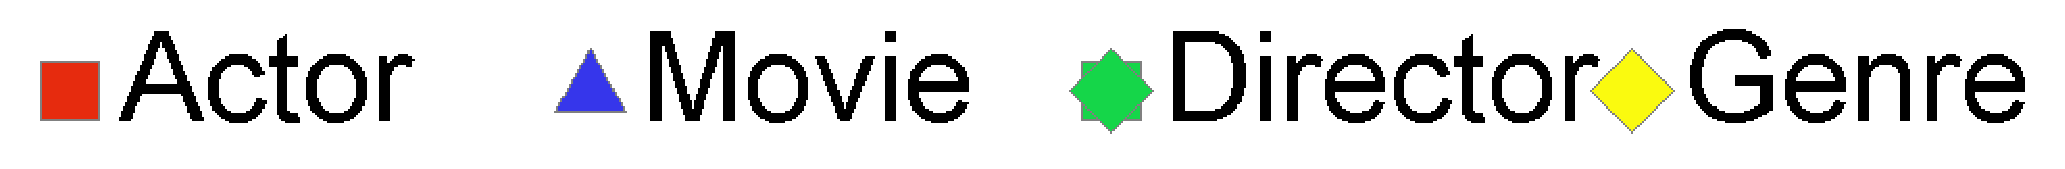
\includegraphics[width=0.45\linewidth]{images/Legends.eps}
	
  \caption{Users' interest in data objects, in relation to each objects' relevance to a task, for twelve tasks of four types. }
	\label{fig:RelevanceDiagram}
\end{figure}



\subsubsection{Viewing Transition Biases Exist and are Significant}
\label{sec:EvalAssumptionAboutViewingTransition}
We performed a quantitative analysis of our subjects' viewing-transition patterns, using the data we collected during our study, and found that the informal assumptions we made in Section~\ref{sec:MehthodsIntelligentAlgorithm} were correct: our users showed strong preferences to view objects that were highlighted or connected to previously viewed objects. The last three columns in Table~\ref{tab:TransitionFromMovie} compare the probability with which our users viewed one object category after another (e.g., viewed a highlighted actor after a movie) as computed from data we collected to a null hypothesis in which users pick at random which items to view next. The quantitative results show for instance that after seeing a movie, our users were four times more likely to look at an actor that was highlighted ($Ratio = 4.081$). Moreover, eleven times more likely to look at an actor that was both highlighted and connected to the previously viewed movie ($Ratio = 11.484$), than if users were viewing items at random.    


To reach these results, we first discarded the prediction component from our data, since it represents exactly the assumption we seek to evaluate. We then counted direct viewing transitions between all types of objects (sources) to all other types of objects (targets) and divided them into categories based on whether targets were highlighted, connected to the sources, or both (Table~\ref{tab:TransitionFromMovie}).  For example, after looking at a movie, our users looked at an actor that was unconnected to that movie and unhighlighted $793$ times, and at an actor that was connect to the movie and highlighted $616$ times. Since in our visualization connections existed only between movies and actors, genres, and directors, transitioning to connected targets was only possible to and from movies.
    

We translated these counts into observed transition probabilities by normalizing them by the total number of transitions from each type of source to each type of category. For example, our users transitioned in total $1784$ times from a movie to an actor, of which $147$ transitions were from a movie to a highlighted actor, yielding an observed transition probability of $147 / 1784 = 0.082$.

However, interpreting these observed probabilities by themselves can be misleading. For example, we observed 793 transitions from a movie to an unconnected actor and just 147 to a connected one. However, This case did not indicate a preference for non-highlighted viewing actors but happened because users had many more opportunities to view unhighlighted actors than they had to view highlighted ones. Intuitively, when a user transitions their gaze from a source to a target, the visualization typically contains many more targets that are not highlighted and are not connected to the source, than those that are. 

Thus, observed transitions should be compared to the default case, which assumes that users treat all visual objects equally. Assume the following simplified case: a movie is connected to two of ten actors shown in a visualization. We observe that of ten transitions from that movie to one of the actors, five were to a connected actor, while five were to unconnected actors. The two observed probabilities, to connected and unconnected actors, would, in this case, be equal at $5/10 = 0.5$. However, if no transitioning preference, the probability of transitioning to any actor would be equal to $0.1$, that of transitioning to a connected actor $0.2$, while that of transitioning to an unconnected actor $0.8$. Thus, our observed transition probability from a movie to a connected actor is $0.5/0.2=2.5$ times higher than the default, unbiased probability, while our observed transition from a movie to an unconnected actor is a fraction ($0.5/0.8=0.625$) of the unbiased one.  

To compute unbiased probabilities, every time we counted a transition from a source to a target, we also counted all target options available to the subject at that point, given the state and structure of the visualization at the time of transition. Reverting to our simplified example, for each of our ten observed transitions we would count two possible transitions to connected actors and eight possible transitions to unconnected actors, ending up with $20$ counts for connected actors, and $80$ counts for unconnected actors. These numbers allow us to compute the two unbiased probabilities as $20/(20+80)$ and $80/(20+80)$.

\begin{table}[htbp]	
\caption{Transitions from a Movie object.}
	\centering
		\begin{tabular}{|c|c|c|c|c|c|}
			\hline
			 \multicolumn{2}{ |c| }{Movie to}  &\shortstack{No. of\\transitions} 	&\shortstack{ Observed \\trans.\\prob. }	&\shortstack{	 Unbiased\\trans.\\prob.} & \shortstack{Ratio \\$\frac{\text{Observed}}{\text{Unbiased}}$}\\ \hline
      \multirow{4}{*}{Actor}	&-	&793	&0.445	&0.898	&0.495	\\	\cline{2-6}
															&H	&147	&0.082	&0.02	&4.081	\\	\cline{2-6}
															&C	&228	&0.128	&0.052	&2.473	\\	\cline{2-6}
															&CH	&616	&0.345	&0.03	&11.484	\\	\hline
				\multirow{2}{*}{Movie}	&-	&5727	&0.761	&0.899	&0.846	\\	\cline{2-6}
																&H	&1798	&0.239	&0.101	&2.376	\\	\hline
				\multirow{4}{*}{Director}	&-	&304	&0.537	&0.887	&0.606	\\	\cline{2-6}
																	&H	&37	&0.065	&0.021	&3.088	\\	\cline{2-6}
																	&C	&51	&0.09	&0.055	&1.647	\\	\cline{2-6}
																	&CH	&174	&0.307	&0.038	&8.176	\\	\hline
				\multirow{4}{*}{Genre}	&-	&193	&0.33	&0.792	&0.417	\\	\cline{2-6}
																&H	&40	&0.068	&0.033	&2.045	\\	\cline{2-6}
																&C	&69	&0.118	&0.102	&1.159	\\	\cline{2-6}
																&CH	&282	&0.483	&0.072	&6.693	\\	
				\hline
		\end{tabular}
		
	\label{tab:TransitionFromMovie}
\end{table}

\begin{table}[htbp]	
\caption{Transitions from Actor objects. }
	\centering
	\begin{tabular}{|c|c|c|c|c|c|}
			\hline
			 \multicolumn{2}{ |c| }{Actor to}    &\shortstack{No. of\\transitions} 	&\shortstack{ Observed \\trans.\\prob. }	&\shortstack{	 Unbiased\\trans.\\prob.} & \shortstack{Ratio \\$\frac{\text{Observed}}{\text{Unbiased}}$}\\ \hline
						 \multirow{2}{*}{Actor}	&-	&4711	&0.685	&0.962	&0.713	\\	\cline{2-6}
																		&H	&2164	&0.315	&0.038	&8.207	\\	\hline
							\multirow{4}{*}{Movie}	&-	&839	&0.469	&0.82	&0.572	\\	\cline{2-6}
																			&H	&213	&0.119	&0.058	&2.046	\\	\cline{2-6}
																			&C	&386	&0.216	&0.076	&2.843	\\	\cline{2-6}
																			&CH	&352	&0.197	&0.046	&4.284	\\	\hline
							\multirow{2}{*}{Director}	&-	&68	&0.701	&0.959	&0.731	\\	\cline{2-6}
																				&H	&29	&0.299	&0.041	&7.271	\\	\hline
							\multirow{2}{*}{Genre}	&-	&43	&0.524	&0.931	&0.563	\\	\cline{2-6}
																			&H	&39	&0.476	&0.069	&6.918	\\	
				\hline
		\end{tabular}
		
	\label{tab:TransitionFromActor}
\end{table}

\begin{table}[htbp]	
\caption{Transitions from Director objects}
	\centering
\begin{tabular}{|c|c|c|c|c|c|}
			\hline
			 \multicolumn{2}{ |c| }{Director to}    &\shortstack{No. of\\transitions} 	&\shortstack{ Observed \\trans.\\prob. }	&\shortstack{	 Unbiased\\trans.\\prob.} & \shortstack{Ratio \\$\frac{\text{Observed}}{\text{Unbiased}}$}\\ \hline
       \multirow{2}{*}{Actor}	&-	&71	&0.747	&0.958	&0.78	\\	\cline{2-6}
															&H	&24	&0.253	&0.042	&5.964	\\	\hline
			\multirow{4}{*}{Movie}	&-	&271	&0.494	&0.792	&0.623	\\	\cline{2-6}
															&H	&55	&0.1	&0.04	&2.478	\\	\cline{2-6}
															&C	&130	&0.237	&0.108	&2.198	\\	\cline{2-6}
															&CH	&93	&0.169	&0.06	&2.841	\\	\hline
			\multirow{2}{*}{Director}	&-	&384	&0.706	&0.93	&0.759	\\	\cline{2-6}
																&H	&160	&0.294	&0.07	&4.216	\\	\hline
			\multirow{2}{*}{Genre}	&-	&256	&0.522	&0.899	&0.581	\\	\cline{2-6}
															&H	&234	&0.478	&0.101	&4.708	\\	
				\hline
		\end{tabular}
		
	\label{tab:TransitionFromDirector}
\end{table}

\begin{table}[htbp]	
\caption{Transitions from Genre objects}
	\centering
	\begin{tabular}{|c|c|c|c|c|c|}
			\hline
			 \multicolumn{2}{ |c| }{Genre to}   &\shortstack{No. of\\transitions} 	&\shortstack{ Observed \\trans.\\prob. }	&\shortstack{	 Unbiased\\trans.\\prob.} & \shortstack{Ratio \\$\frac{\text{Observed}}{\text{Unbiased}}$}\\ \hline
			 \multirow{2}{*}{Actor}	&-	&61	&0.656	&0.9791	&0.67	\\	\cline{2-6}
															&H	&32	&0.344	&0.021	&16.47	\\	\hline
				\multirow{4}{*}{Movie}	&-	&229	&0.118	&0.261	&0.453	\\	\cline{2-6}
																&H	&46	&0.024	&0.008	&3.001	\\	\cline{2-6}
																&C	&172	&0.089	&0.093	&0.956	\\	\cline{2-6}
																&CH	&138	&0.071	&0.013	&5.288	\\	\hline
				\multirow{2}{*}{Director}	&-	&282	&0.591	&0.973	&0.608	\\	\cline{2-6}
																	&H	&195	&0.409	&0.027	&15.174	\\	\hline
				\multirow{2}{*}{Genre}	&-	&348	&0.398	&0.943	&0.422	\\	\cline{2-6}
																&H	&526	&0.602	&0.057	&10.627	\\	
				\hline
		\end{tabular}		
		
	\label{tab:TransitionFromGenre}
\end{table}
%\begin{table}[htbp]	
	%\centering
		%\begin{tabular}{|c|c|c|c|c|c|}
			%\hline
			 %\multicolumn{2}{ |c| }{Movie to}  &\shortstack{No. of\\transitions} 	&\shortstack{ Observed \\trans.\\prob. }	&\shortstack{	 Unbiased\\trans.\\prob.} & \shortstack{Ratio \\$\frac{\text{Observed}}{\text{Unbiased}}$}\\ \hline
      %\multirow{4}{*}{Actor}	&-	&793	&0.445	&0.898	&0.495	\\	\cline{2-6}
															%&H	&147	&0.082	&0.02	&4.081	\\	\cline{2-6}
															%&C	&228	&0.128	&0.052	&2.473	\\	\cline{2-6}
															%&CH	&616	&0.345	&0.03	&11.484	\\	\hline
				%\multirow{2}{*}{Movie}	&-	&5727	&0.761	&0.899	&0.846	\\	\cline{2-6}
																%&H	&1798	&0.239	&0.101	&2.376	\\	\hline
				%\multirow{4}{*}{Director}	&-	&304	&0.537	&0.887	&0.606	\\	\cline{2-6}
																	%&H	&37	&0.065	&0.021	&3.088	\\	\cline{2-6}
																	%&C	&51	&0.09	&0.055	&1.647	\\	\cline{2-6}
																	%&CH	&174	&0.307	&0.038	&8.176	\\	\hline
				%\multirow{4}{*}{Genre}	&-	&193	&0.33	&0.792	&0.417	\\	\cline{2-6}
																%&H	&40	&0.068	&0.033	&2.045	\\	\cline{2-6}
																%&C	&69	&0.118	&0.102	&1.159	\\	\cline{2-6}
																%&CH	&282	&0.483	&0.072	&6.693	\\	
				%\hline
		%\end{tabular}		
		%\caption*{(a)Transitions from Movies}
		%\smallskip
		%
		%\begin{tabular}{|c|c|c|c|c|c|}
			%\hline
			 %\multicolumn{2}{ |c| }{Actor to}    &\shortstack{No. of\\transitions} 	&\shortstack{ Observed \\trans.\\prob. }	&\shortstack{	 Unbiased\\trans.\\prob.} & \shortstack{Ratio \\$\frac{\text{Observed}}{\text{Unbiased}}$}\\ \hline
						 %\multirow{2}{*}{Actor}	&-	&4711	&0.685	&0.962	&0.713	\\	\cline{2-6}
																		%&H	&2164	&0.315	&0.038	&8.207	\\	\hline
							%\multirow{4}{*}{Movie}	&-	&839	&0.469	&0.82	&0.572	\\	\cline{2-6}
																			%&H	&213	&0.119	&0.058	&2.046	\\	\cline{2-6}
																			%&C	&386	&0.216	&0.076	&2.843	\\	\cline{2-6}
																			%&CH	&352	&0.197	&0.046	&4.284	\\	\hline
							%\multirow{2}{*}{Director}	&-	&68	&0.701	&0.959	&0.731	\\	\cline{2-6}
																				%&H	&29	&0.299	&0.041	&7.271	\\	\hline
							%\multirow{2}{*}{Genre}	&-	&43	&0.524	&0.931	&0.563	\\	\cline{2-6}
																			%&H	&39	&0.476	&0.069	&6.918	\\	
				%\hline
		%\end{tabular}
	%\caption*{(b)Transitions from Actors}
	%\smallskip
	%
	%\begin{tabular}{|c|c|c|c|c|c|}
			%\hline
			 %\multicolumn{2}{ |c| }{Director to}    &\shortstack{No. of\\transitions} 	&\shortstack{ Observed \\trans.\\prob. }	&\shortstack{	 Unbiased\\trans.\\prob.} & \shortstack{Ratio \\$\frac{\text{Observed}}{\text{Unbiased}}$}\\ \hline
       %\multirow{2}{*}{Actor}	&-	&71	&0.747	&0.958	&0.78	\\	\cline{2-6}
															%&H	&24	&0.253	&0.042	&5.964	\\	\hline
			%\multirow{4}{*}{Movie}	&-	&271	&0.494	&0.792	&0.623	\\	\cline{2-6}
															%&H	&55	&0.1	&0.04	&2.478	\\	\cline{2-6}
															%&C	&130	&0.237	&0.108	&2.198	\\	\cline{2-6}
															%&CH	&93	&0.169	&0.06	&2.841	\\	\hline
			%\multirow{2}{*}{Director}	&-	&384	&0.706	&0.93	&0.759	\\	\cline{2-6}
																%&H	&160	&0.294	&0.07	&4.216	\\	\hline
			%\multirow{2}{*}{Genre}	&-	&256	&0.522	&0.899	&0.581	\\	\cline{2-6}
															%&H	&234	&0.478	&0.101	&4.708	\\	
				%\hline
		%\end{tabular}
		%\caption*{(c)Transitions from Director}
		%\smallskip
		%
		%\begin{tabular}{|c|c|c|c|c|c|}
			%\hline
			 %\multicolumn{2}{ |c| }{Genre to}   &\shortstack{No. of\\transitions} 	&\shortstack{ Observed \\trans.\\prob. }	&\shortstack{	 Unbiased\\trans.\\prob.} & \shortstack{Ratio \\$\frac{\text{Observed}}{\text{Unbiased}}$}\\ \hline
			 %\multirow{2}{*}{Actor}	&-	&61	&0.656	&0.9791	&0.67	\\	\cline{2-6}
															%&H	&32	&0.344	&0.021	&16.47	\\	\hline
				%\multirow{4}{*}{Movie}	&-	&229	&0.118	&0.261	&0.453	\\	\cline{2-6}
																%&H	&46	&0.024	&0.008	&3.001	\\	\cline{2-6}
																%&C	&172	&0.089	&0.093	&0.956	\\	\cline{2-6}
																%&CH	&138	&0.071	&0.013	&5.288	\\	\hline
				%\multirow{2}{*}{Director}	&-	&282	&0.591	&0.973	&0.608	\\	\cline{2-6}
																	%&H	&195	&0.409	&0.027	&15.174	\\	\hline
				%\multirow{2}{*}{Genre}	&-	&348	&0.398	&0.943	&0.422	\\	\cline{2-6}
																%&H	&526	&0.602	&0.057	&10.627	\\	
				%\hline
		%\end{tabular}
		%\caption*{(d)Transitions from Genres}\smallskip
	%\captionof{table}{Transitions from a source object to a target object, divided by: (i) type of source and target; (ii) whether the target was highlighted (H); (iii) whether the target was highlighted and connected to the source (HC); (iv) and whether source and target were neither highlighted nor connected. Columns show: (i) the number of direct transitions for the source/target combination; (ii) the observed transition probability from the source to that target; (iii) the (unbiased) probability of transition between source and target if all elements had equal probability to be viewed; (iv) the ratio between observed and unbiased transition probabilities.}
	%\label{tab:TransitionFromMovie}
%\end{table}

\section{Conclusion}
\label{sec:DOICollectionConclusion}
In visualizations that are open to instrumentation, gaze information provided by an eye-tracker can be used to automatically detect what visual objects users are likely to be viewing. Such detection can provide results that are almost as accurate as annotations created by human coders, provided that detection is done ``intelligently'', by using gazes together with a prediction of which objects are likely to be viewed at a given time. Data collected in this way is highly granular and has semantic content because it is linked to the data underlying the visualization. For this reason, and because it does not require any human pre-processing, object viewing data can be collected and analyzed efficiently for many subjects, using interactive visualizations, for long analytic session, and could be used in studies that explore how analysts hypothesize about data using complex visual analytics systems. 




\chapter{CASE STUDIES}
\label{chap:CaseStudies}

In this chapter, we explore the use of the DOI methodology in three concrete projects. We report on the instrumentation process, the data collection methods, and the research goals of these projects as a means of exemplifying the research processes that the DOI approach can facilitate.  

\section{Tracking Data Consumption in Visualization Systems}
\label{sec:ExperimentIMDB}
We study the degree to which the DOI approach can enable visualization researchers and analysts to track and understand what data users are foraging for, and what types of questions they are trying to answer while using interactive visualization systems. We showed that DOI data could reveal to an analyst, even in real-time, details about the tasks users are pursuing in an interactive visualization~\cite{Ala16, alam2015they}. We used this experiment to evaluate our first contributions (i.e. Section~\ref{sec:DOICollectionEvaluation}). 

To drive this research, we instrumented a Java-based PivotPaths~\cite{Dor12} visualization of movie data from the Internet Movie Database (IMDB). The visualization showed actors, movies, directors, and genres as 2D nodes connected by curves and was interactive. It could be zoomed and panned, users could select and highlight data, and could change the subset of data shown at any given time. 

We instrumented the visualization by inserting instructions that mirrored its modeling and rendering code so as to inform a viewed object detection module of the shapes, positions, and attributes (e.g., actor name, age, gender) of objects shown on the screen at any given time. We tracked individual data items (e.g., actor). The object detection module matched 2D gaze points received from an eye-tracker to screen objects reported by the visualization. We collected data from $9$ subjects using these visualizations interactively for thirty to forty-five minutes. The experimentation and instrumentation process is described in detail in Chapter~\ref{chap:DOIDataCollection}.

Typical questions we found that we were able to answer from DOI data were: ``Did a user try to solve a given task, or did they focus on specific data?'', ``Did a tracked user switch their analysis focus?'', ``When did a tracked user start solving a specific task?'', ``What data did users focus on when asked to solve a particular task?''. Such analyses can advance the visual analytics agenda by providing unprecedented insights into how users forage for and analyze data naturally, in interactive visual analytics systems and over extended periods of time. 

\section{Understanding Student Learning}
\label{sec:ExperimentArchitecture}
We work with education researchers to understand how students learn architecture using visual, interactive instruction material. In a preliminary pilot study with six subjects, we found that we can collect detailed DOI data from students learning via an interactive learning environment, to reveal the type of content learners focus on, and the sequences and patterns in which they do so. 

We explored an existing learning environment designed to teach architecture concepts related to facades and energy efficient building materials. This learning module was structured as an informational web application (HTML + Javascript), contained primarily text and images, and was interactive in that students could navigate between learning concepts, collapse and expand sections, and obtain details on demand. 

As described before, we instrumented the HTML and javascript code to allow the learning environment to permanently communicate (via AJAX protocols) to a viewed object detection module the shape, position, and nature (i.e., attributes) of the content it showed on the screen at any moment in time. As part of our experimental setup, students interacted with the web content on a local machine that we equipped with an eye-tracker. The detection module received gaze data from the eye-tracker and matched it to the visual content reported by the learning environment, to identify and record likely viewing targets.

Individual DOM elements with sufficient semantic meaning (e.g., paragraphs, images, headers, navigation widgets) formed the basis of DOI elements (Figure~\ref{fig:archictecture}). In Figure~\ref{fig:archictecture}, we depict our instrumentation using our DOI method from Chapter~\ref{chap:DOIDataCollection}. The overlays in the figure illustrate defined DOIs. However, several images depicted complex schematics or included multiple panels. In such cases, we defined more granular DOIs within those pictures. 

We annotated DOIs with attributes such as which learning concept the DOI was referring to (e.g., facade, heat transmission, material type). Moreover, its complexity level (introductory, medium, advanced), the type of visual content it was depicted with (e.g., text, image, navigation widget), and the type of learning content (e.g., definition, example, exercise). The learning environment communicated These attributes to the instrumentation library, which in turn stored them as part of the description of viewed objects.

In our pilot experimental setup, six students spent approximately forty-five minutes exploring freely and absorbing the content illustrated in the learning module, as their gazes were tracked. In the end, their learning was quantified using a relatively short multiple choice questionnaire. Additionally, we collected information about students' educational background (e.g., pursued a major, career interests), degree progress (sophomore, junior, senior), and general demographic profile (e.g., age, gender).

This experimental setup and data collection process were designed to allow our collaborators to answer several high-level research questions expressed at our project's outset. These include: "Does a particular type or learning content or viewing pattern correlate with more efficient learning?"; "Does student background (e.g., engineering, science, arts) correlate with the type of content students focus on?"; "Are there viewing patterns that can predict learning deficiencies?". We hypothesize that the highly granular and annotated DOI data collected over extended periods of time from students learning "in the wild" from interactive visual content will facilitate insight different than that enabled by typical AOI-driven eye-tracking analyses.

\begin{figure}[htbp]
  \centering
  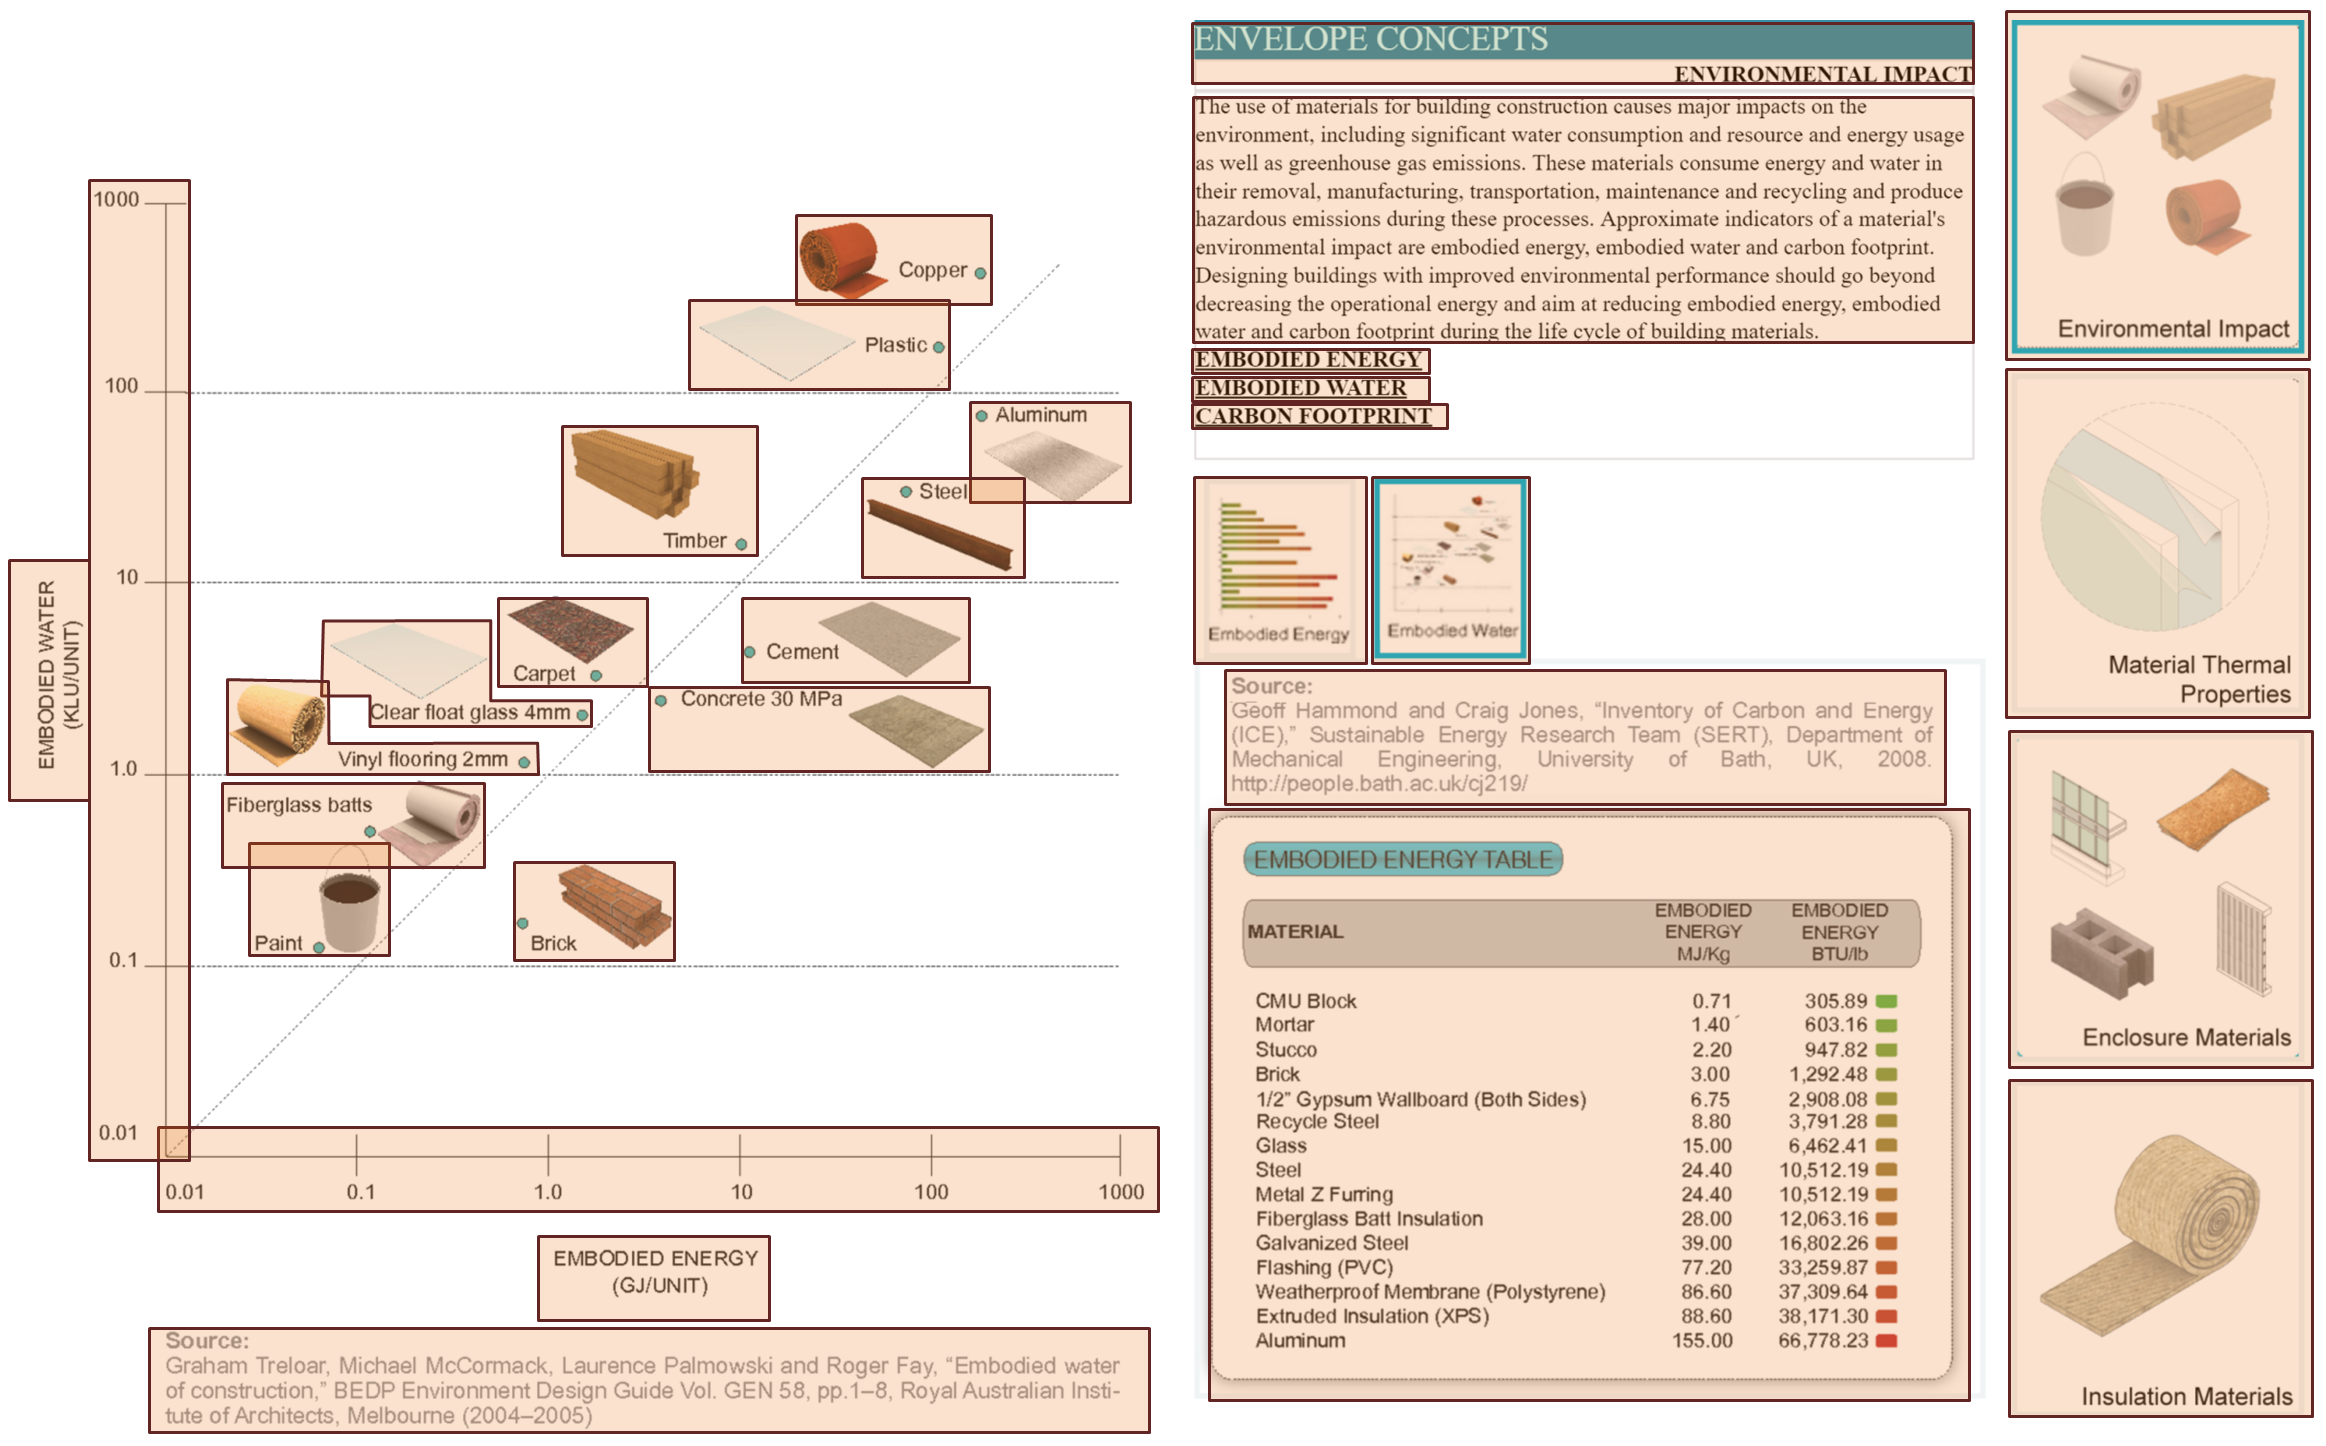
\includegraphics[width=\linewidth]{images/architectureDOI.eps}
  \caption{A single page of an interactive, HTML environment for learning architecture concepts.}
	\label{fig:archictecture}
\end{figure}

\section{Exploring How Workers Detect and Assess Hazardous Situations on Construction Scenes}
\label{sec:ExperimentConstruction}
We collaborate with civil engineering researchers wishing to understand and model how construction workers identify and respond to safety hazards in construction scenes. Such research is important as the construction industry  suffers from the highest  number of  occupational fatalities  among all  the industries. 

Existing studies have explored the visual perception of workers on construction sites by tracking workers' gazes as they observe active sites for specific amounts of time~\cite{SafetyPerf}. However, simulating hazardous scenarios in-vivo is at best difficult, if not impossible. 
Moreover, capturing and analyzing eye-tracking data for videos is laborious, thus limiting previous experiments to short, constrained scenarios. 

Instead, we modeled a 3D construction scene from a real scene, using the Unity 3D framework, and had subjects explore this scene virtually on a computer screen, while an eye-tracker, in lieu with DOI instrumentation, captured which construction elements they observed. 

The scene was dynamic and involved multiple unfolding hazardous situations (e.g., a construction worker rushing in front of a vehicle). Subjects were assigned a virtual character which the scene placed in a truck that moved along a predetermined path through the scene (Figure ~\ref{fig:construction}). Subjects had no control over the transition of the camera (i.e., the truck's path), but they could change their viewing angle by rotating the camera in the horizontal plane. The whole 'trip' through the construction scene lasted approximately $8$ minutes. 

We instrumented the Unity scene using Bernhard et al.'s GTOM approach~\cite{Bern14}. Specifically, in addition to rendering the scene on the screen for subjects to view, we assigned each tracked object a specific color and rendered objects into a color buffer. We then identified colors in the proximity of gaze coordinates supplied by the eye-tracker and used this information to detect objects subjects potentially viewed. Figure~\ref{fig:construction} illustrates an example of the process. Each 3D object tracked in the scene is projected in the color buffer using a distinct color. Gazes are mapped to objects in the 3D space via their colors in the buffer.

Through the instrumentation process, we exported object attributes such as type (e.g., machinery, human, static), hazards associated with each object (e.g., collision, electrocution), whether objects were moving or not,  and their distance from the subject's camera. At the same time, we used the color buffers to compute the size of objects and their position (i.e., the center of mass) on the screen, and we tracked which of all objects were visible and which not. We note that the latter five types of attributes were time dependent. We also recorded screen captures and computed the bounds of objects on the screen. 

We collected such DOI data from sixteen subjects, half of which had construction training and the half which had not. Subjects were asked to complete a post-questionnaire about which hazardous situations they detected. Additionally, we collected subject-specific information such as experience and training levels. 

Specific questions that our collaborators expressed interest in, and that this experimental setup was designed to answer, included ``Viewing which types of visual items lead workers to identify specific hazards?'', ``How does the interest of experienced and novice construction workers in construction scene elements differ?'', ``Are there any low-level visual patterns that are unique to experienced construction workers?'', moreover, ``What types of hazards might go unnoticed at a construction site?''.

In addition to enabling the study of hazardous situations that are not safe to reproduce in vivo, we hypothesize that this DOI approach will eventually facilitate a novel, data-driven experimentation process. Specifically, our collaborators will be able to alter the construction scene often, between participant groups and in response to subjects' actions, or to simulate varied types of hazards and construction scene configurations, and document the resulting visual behavior. Examples of alterations include removing a virtual worker's reflective vest, altering the path of a worker to lead through a dangerous area, and removing or adding warning signs. Such experimentation can thus lend more significant data than traditional eye-tracking experimentation and facilitate novel workflows. While it is true that data collected in this way is of less ecological validity than that collected in situ, initial studies have shown that viewing patterns captured in virtual scenes may approximate those captured in real scenes well~\cite{nipesh}.

\begin{figure}[htbp]
  \centering
  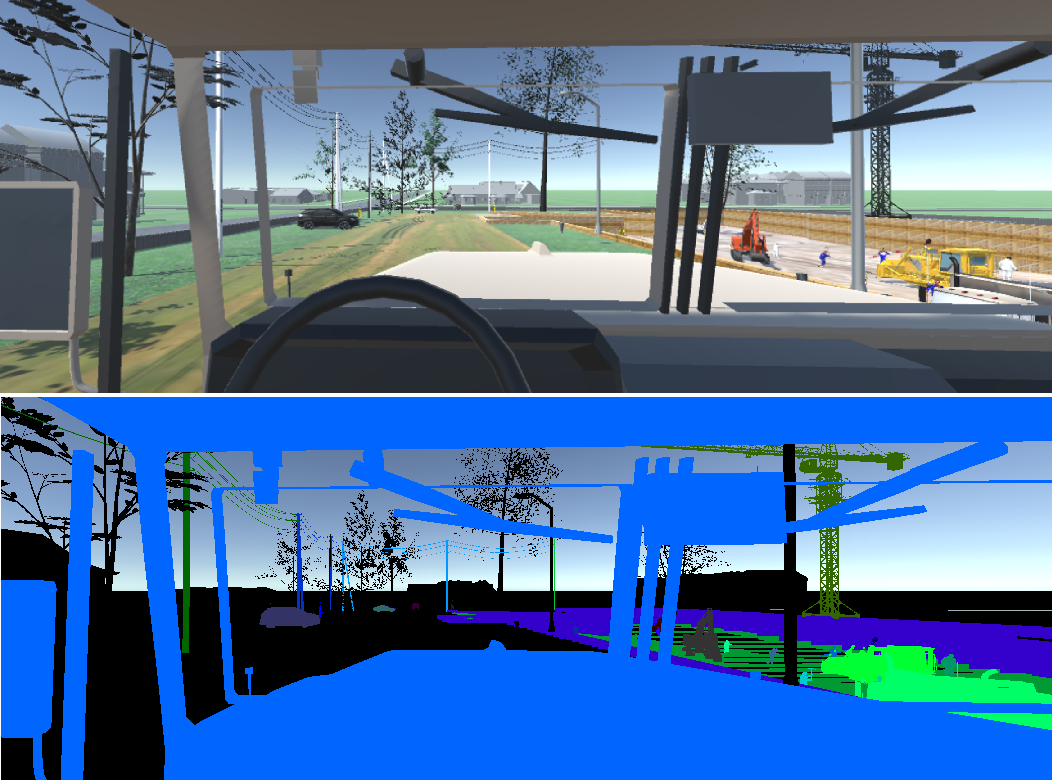
\includegraphics[width=\linewidth]{images/construction.eps}
  \caption{A 3D construction scene model (top) instrumented using Bernhard et al.'s color-buffer (bottom) approach~\cite{Bern14}. }
	\label{fig:construction}
\end{figure}

\section{Conclusions}
The analysis scope of eye-tracking data in any projects can be unbounded. Using real concepts have facilitated us on developing DOI analysis model and methods. All of the three projects mentioned in this chapter (Section~\ref{sec:ExperimentIMDB},~\ref{sec:ExperimentArchitecture}, and~\ref{sec:ExperimentConstruction}) have a general structure. Thus, many data analysis projects can relate to them. In this chapter, we discussed research workflow, analysis scope, visualization, and instrumentation methods. We will refer these projects as a basis for developing DOI data models and analysis framework in the following chapters. 
\chapter{DOI FORMALIZATION: DATA MODEL AND ANALYTIC QUESTIONS}
\section{Introduction}
Due to the differences between DOI and AOI, methods for visualizing and analyzing AOI data are unsuited for the analysis of DOI data. The differences are due to two factors. First, DOIs can be more granular and DOI data much larger compared to AOIs. For example, an eye-tracking visualization instrumented with DOI can track 100 DOIs per frame. Conversely, experimenters are able to annotate only about 10-20 AOIs manually. Thus, AOI-based visualizations are not able to show the typically large volumes of DOI data. For example, Figure~\ref{fig:Scanpath} illustrates a scanpath, a typical AOI visualization,  build from a full DOI dataset including 108 tracked DOIs (Figure~\ref{fig:Scanpath}(a)) and one build from only twelve DOIs (Figure~\ref{fig:Scanpath}(b)), a count more typical of traditional AOI analyses. Both diagrams are generated from an eye-tracking session of ten minutes. It is evident that the scanpath diagram for the full DOI set is more complicated than that representative of AOI analyses. Thus, interpreting large DOI data from such diagram is difficult. 

\begin{figure}[htb]
  \centering
  \includegraphics[width=0.99\linewidth]{images/Scanpath.eps}
  \caption{: Two examples of scanpath visualization. Here, (a) displays scanpath with 108 DOIs. (b) displays scanpath with 12 AOIs. }
	\label{fig:Scanpath}
\end{figure}

\begin{table}[htbp]
	\centering
		\begin{tabular}{|c|c|c|c|}
				\hline
				\textbf{Character}	& \textbf{Survives} &	\textbf{Gender}	& \textbf{Centrality}\\\hline
			
				Valjean	& No	&Male	&1\\\hline
Javert	&No&	Male&	3\\\hline
Cosette 	&Yes	&Female&	2\\\hline
Marius	&Yes	&Male&	6\\\hline
Eponine	&No	&Female&	4\\\hline
Fantine	&No	&Female	&5\\\hline
Thanerdier	&Yes	&Male	&7\\\hline

		\end{tabular}
		\caption{Two attribute (isAlive,Gender, and Centrality) data for each character in the Les Miserables Data. }
		\label{tab:LesMiserablesAttribute}
\end{table}

Second, since DOIs are derived from data, they have explicit attributes. Each DOI is described by a set of attributes that the visualization can access, display, and leverage. Instead, AOIs have implicit attributes that only experimenters that defined them know. Such attributes are inaccessible to visualizations and analysis software. For example, consider that in `The Les Miserables Visualization' example (Figure~\ref{fig:MiserablesSimple}), each character is described by attributes (Table~\ref{tab:LesMiserablesAttribute}) such as `Centrality', `Gender' and `Survives' (i.e. whether the character is alive at the end of the novel). Once they collect data about which objects subjects viewed, analyzers can answer a breadth of questions such as ``Are users more likely to view female characters rather than male characters?'', ``Are users more likely to view deceased characters rather than alive?'', or ``Do users tend to look at central characters?''. 

In conclusion, DOI data interpretation is different than AOI data. Hence, we aim to formalize DOI data model and analysis tasks. In this chapter, we discuss our contributions of a general data model in Section~\ref{sec:DOIDataModel} and list of analysis questions for DOI data in Section~\ref{sec:DOIAnalysisTasks}. Moreover, we discuss a comparison between AOI and DOI data in Section~\ref{sec:AOIvsDOI}. Finally, we conclude our discussion about this chapter in Section~\ref{sec:DOIAnalysisModelConclusion}.



\section{General DOI Data Model}
\label{sec:DOIDataModel}
As described in Chapter~\ref{chap:Intro}, peoples' foveas are guided by visual cues in perceived scenes. To study how people parse a scene, especially from a perceptual (bottom-up) perspective, access to the visual attributes of objects in it (e.g., color, movement) is indispensable. However, visual attributes often encode semantic properties of data (e.g., color may encode disease type in a medical visualization). To hypothesize about cognitive and goal-directed processes that drive visual ones, analysts may wish to investigate directly what data people looked at, as opposed to how the data was shown. This aligns with the top-down theory of visual processing, which implies that it is meaning and significance of content, together with representation, that drives visual scanning. The DOI approach is to capture both visual and semantic data from eye-tracking experiments to support various research questions, such as about perception, cognition, or data exploration and search. 

DOIs are defined to overlap significant chunks of a visualization's underlying data (e.g., a protein in a protein-interaction network), and inherit the semantic data attributes and values that define those chunks (e.g., protein name, type, function). DOIs also include visual attributes that describe how that information is shown on the screen (e.g., shape, the color of protein glyph). A DOI instrumentation will capture for each user fixation; the DOIs the user may have intended to view, potentially along with low-level attributes of the respective fixation. Below we describe a formal model that captures this idea, and exemplify it in the context of the three case studies (Table~\ref{tab:DOIDataExamples}).

We approximate a visualization's data using the generic entity-attribute-value (EAV) data model~\cite{deran1991entity}, in which combinations of attribute-value pairs describe entities.  We thus define data as the set $D$, containing $N\!d$ data entities $d$. Each entity is itself defined by multiple pairs of data attributes ($da$) and data attribute values ($dav$):
%%\vspace{-0.5mm}
\begin{equation*}
\begin{split} 
D = \{d_i \,|\, i=1..N\!d\} \\
d_{i} = \{da_{i,k} = dav_{i,k} \,|\, k=1..N\!da_{i}\}
\end{split}
\end{equation*}

The definition above describes static datasets. In real applications, data can change over time as a result of user interaction (e.g., a user changes the speed of a vehicle in a 3D simulation; user annotates or deletes data in a visualization). Again, as a result of factors external to the visualization (e.g., data is streamed from a simulation). We augment the definition to include a temporal domain $T$ (e.g., the time of the eye-tracking experiment):
%%\vspace{-0.5mm}
\begin{equation*}
\begin{split}
D_t = \{d_{i,t} \,|\, i=1..N\!d_t, t \in T\} \\
d_{i,t} = \{da_{i,t,k} = dav_{i,t,k} \,|\, k=1..N\!da_{i,t}\}
\end{split}
\end{equation*}

Visualizations turn data sets into visual models by defining visual elements to represent data elements. While this mapping is often one to one, this is not necessarily true; a single visual representation might capture multiple data elements. As such, we will define a visual model as the set $M$, containing $N\!m$ visual entities $m$. Each visual entity contains a reference to one or more data entities it depicts, and a collection of visual attributes and values that define it (e.g., position, shape, size, color). As before, our definition accounts for possible changes over time, as users may change a visualization through interaction.  

\vspace{-4mm}
\begin{multline*}
\qquad\qquad\quad\; M_t = \{m_{i,t} \,|\, i=1..N\!m_t, t \in T\} \\
m_{i,t} = \{\,\{d_{j,t}\,|\, j=1..N\!md_{i,t}\}, \\ ma_{i,t,k} = mav_{i,t,k} \,|\, k=1..N\!ma_{i,t}\}
\end{multline*}

Finally, models are rendered on the screen via a transformation (e.g., dependent on zooming and panning in 2D visualizations) or projection (e.g., dependent on perspective changes in 3D). The mapping between model and screen entities is generally one to one (i.e., one screen entity for each model entity), but attribute values may differ between model and screen entities even when attribute names are similar. For example, an entity's size in model space is often not the same as in screen space. So, we define our screen visualization as a set of screen entities, same in number as model entities, with one associated model entity, and pairs of screen attributes and values. Screen attributes can include screen-capture cutouts of individual DOIs.

\vspace{-3mm}
\begin{multline*}
\qquad\qquad\; S_t = \{s_{i,t} \,|\, i=1..N\!m_t, t \in T\} \\
s_{i,t} = \{m_{i,t}, \,\, sa_{i,t,k} = sav_{i,t,k} \,|\, k=1..N\!sa_{i,t}\}
\end{multline*}

Eye-trackers report fixations periodically, as time-stamped 2D coordinates with an associated duration. Fixations may be described by additional properties such as dispersion or pupil size.So, we define fixations reported during an experiment as:

\vspace{-5mm}
\begin{multline*}
F_t = \{x, y, duration, fa_{k} = fav_{k} \, | \, k=1..N\!fa_t\}, \, t \in T
\end{multline*}

Both Bernhard et al.~\cite{Bern14} and our method (Chapter~\ref{chap:DOIDataCollection}) compute candidate objects a user is likely to have viewed during a fixation by considering not just the fixation point, but also a small area around it. If multiple DOIs intersect that area, Bernhard et al. report only the object closest to the fixation, while our method report all viewing candidates.  For a more general DOI data model, we will consider the approach we discussed in Chapter~\ref{chap:DOIDataCollection}. Thus, each fixation may be associated with multiple viewed DOIs, and the confidence that a DOI was indeed the locus of a user's attention is proportional to the proximity of the fixation to the DOI (Chapter~\ref{chap:DOIDataCollection}). For maximum flexibility, DOI instrumentations can record the distance of users' fixations to all DOIs, postponing its interpretation (i.e., should an object be considered viewed or not viewed given a specific distance) until the analysis stage: 


$$
d(\,F_t, s_{i,t}\,) = 
\begin{cases}
pixels\,from\,F\,to\,center\,or\,border\,of\,s, & \\ \qquad if\,s\, is \, visible\,on\,screen \\ 
\infty \, , \, otherwise 
\end{cases}
$$

This definition allows us to capture not just DOIs users viewed in an experiment, but also which DOIs were visible and not visible during the experiment and when. This allows analysts to understand not just what viewers chose to view, but also what they chose to ignore. 

Finally, a typical eye-tracking experiment captures DOI sequences for multiple users, as well as data describing those users individually. Since through interaction users can change both the data and how it is displayed, all already introduced definitions should be augmented to reflect that they are user specific. User data ($U$) includes for each user ($u_i$) background and demographic information (e.g., education background, level of expertise, gender), but also user performance data (e.g., answers to questionnaires). Such user attributes could be time dependent (e.g., self-reported fatigue):

\vspace{-5mm}
\begin{equation*}
\begin{split}
U_t = \{u_{i,t} \,|\, i=1..N\!u_t, t \in T\} \\
u_{i,t} = \{ua_{i,t,k} = uav_{i,t,k} \,|\, k=1..N\!ua_{i,t}\}
\end{split}
\end{equation*}

Using the definitions introduced above, DOI data can be formallly described as: 

\vspace{-5mm}
\begin{multline*}
DOI_{t,u} = \{S_{t,u} (+\,linked\, M, D), \\ d(F_{t,u}, S_{t,u}), F_{t,u}, u_{u,t}\} \,|\,t \in T, u = 1..N\!u
\end{multline*}

That is, DOIs are analytic constructs that overlap data elements or subsets and are characterized by four types of attributes: data, visual, user, and perceptual. Examples are shown in Table~\ref{tab:DOIDataExamples}. 
These attributes may be time and user dependent, capturing that in real-life visualizations data and visual encoding change in response to user interactions and external factors.  The model defines data that can be collected in an eye-tracking experiment exhaustively and can thus underlie a broad range of research questions. Visual attributes can reveal the perceptual mechanisms that compel peoples' foveas to fixate on specific visual objects (bottom-up perception). Data attributes may better reveal why users intently choose to look at particular data, and could provide insight into cognitive processes associated with top-down perception. User attributes can tie perceptual and cognitive patterns to user demographics, abilities, and performance. Moreover, the model can be extended as necessary with additional types of attributes, such as modality (e.g., audio) or interaction annotations (e.g., is an object the target of an interaction).

%
\begin{table}[htbp]	
	\centering
    \begin{tabular}{|c|c|c|}
    \hline
    Visual Analytics & Learning Education & Construction \\\hline
    DOI (at fixation $N$) & DOI (at fixation $N$) &DOI (at fixation $N$)\\
    \begin{tabular}{l}
         \textbf{data attributes}\\
                 type       :  movie\\
            label   :  The Dark Knight\\
            rating: $9.0$\\
     \textbf{visual attributes}\\
                visible : yes\\
                pos      :  $550,300$ (px) \\
                size      :  $200,150$ (px)\\
     \textbf{user attributes}\\
                id                   :  user1  \\
                level              :  graduate\\
                background :  computer science\\
                
    \textbf{perceptual attributes}\\
                fix\_pos       : $450,280$ (px)\\
                fix\_spread : $30,25$ (px)\\
                distance     : $20$ (px)\\
                time            : $720,000$ (ms)\\
                duration     : $300$ (ms)
	\end{tabular}
    & 
    \begin{tabular}{l}
         \textbf{data attributes}\\
                type       :  definition\\
                format   :  text\\
                concept :  structure\\
                level       :  intro\\
     \textbf{visual attributes}\\
                visible : yes\\
                pos      :  $120,300$ (px) \\
                size      :  $300,100$ (px)\\
     \textbf{user attributes}\\
                id                   :  user1  \\
                level              :  senior\\
                background :  arts\\
                accuracy       :  85 ($\%$)\\
    \textbf{perceptual attributes}\\
                fix\_pos       : $130,280$ (px)\\
                fix\_spread : $30,25$ (px)\\
                distance     : $20$ (px)\\
                time            : $51,000$ (ms)\\
                duration     : $280$ (ms)
	\end{tabular}
    &
    \begin{tabular}{l}
     \textbf{data attributes}\\
            type       :  worker\\
            helmet   :  yes\\
            size         : $0.7,0.4,1.8$ (m)\\
            moving :  $1.5$ (m/s)\\
            hazard  :  caught in between\\
 \textbf{visual attributes}\\
            visible              :  yes\\
            pos                   :  $560,430$ (px) \\
            size                   :  $20,40$ (px)\\
            color                :  $(100,150,150)$\\
            appearance    :  image ref\\
 \textbf{user attributes}\\
            id                   :  user1  \\
            experience   : $5$  (years) \\
            background :  construction\\
            accuracy       :  $7$ (hazards spotted)\\
\textbf{perceptual attributes}\\
            fix\_pos       : $130, 280$ (px)\\
            fix\_spread : $30,25$ (px)\\
            distance     : $20$ (px)\\
            time            : $51,000$ (ms)\\
            duration     : $280$ (ms)
\end{tabular}\\
\hline
	\end{tabular}
    \vspace{3mm}
    
	\caption{Example DOIs and attributes collected in each of the three applications described in Chapter~\ref{chap:CaseStudies}.}
    \label{tab:DOIDataExamples}
\end{table}
\section{Possible and Probable DOI Tasks}
\label{sec:DOIAnalysisTasks}

\subsection{Related Work}
AOI analysis task categorization is non-existent. In this section, we discuss related works on contributions regarding task taxonomies and frameworks and draw inspiration from the methods involved in their creation. We primarily focus on task taxonomies for spatio-temporal data by Andrienko et al.~\cite{And03}, and cartography and geo-visualization by Roth~\cite{Roth13}. Similar to these works, we aim to generate and categorize DOI tasks by considering data-derived goals (i.e., high-level, domain-specific questions that analysts would like to answer), operands (i.e., the specification and answer of a data question), and objectives (i.e., low-level analytic question on the data). 

Previous efforts found it useful to define tasks regarding their operands, data categories that can be used as inputs (i.e., task specification) and outputs (i.e., answer) to a task.  For example, in the context of geographical data, Andrienko et al. defined three basic operands: space (where), time (when), and object (what). Using these operands, Andrienko et al.'s defined three basic kinds of possible questions, regarding inputs and outputs, for spatio-temporal analyses: $when + where \rightarrow what$, $when + what \rightarrow where$, and $where + what \rightarrow when$. We aim to employ a similar analysis in the context of the formal DOI data model. Therefore, an example of a ($when + where \rightarrow what$) question in our particular domain could be ``Which character (What) was viewed in Time T (When) in `Fantine Cluster' (Where) in the Les Miserables Graph (Figure~\ref{fig:Miserables})?''. However, our data model is likely to differ from that of Andrienko (e.g., by including different types of operands), and as such the space of possible tasks will differ as well. 

Additionally, existing work also found it useful to define tasks regarding their objective primitives, or what type of cognitive task they involve. For example, Roth's five objective primitives include: identify (i.e., find a piece of information given some other piece of information), compare (i.e., compare two pieces of information at the same time), rank (i.e. determine order of information pieces), associate (i.e. capture relationships between different information pieces), and delineate (i.e. group or cluster information pieces)~\cite{Roth13}.  Roth's objective primitives are validated empirically and are thus well suited to categorize both loosely defined and specific objectives. We combined these objectives with our operand models to define the possible range of possible DOI tasks. For example, a specific task involving these operands and this objective would be ``Which character was viewed most (objective: rank) by user A (operand: who)?''. 

\subsection{Objectives and Probable Data Questions}
After reviewing multiple taxonomies and frameworks, we decided to use Roth's five objective primitives --- \textit{identify, compare, rank, associate, delineate} ~\cite{Roth13}  --- for two reasons. First, these targets were validated empirically and shown to correlate with how real users think about the tasks they are doing. Second, they are a compromise between loosely defined objectives with a broad meaning and very specific targets. For example, Andrienko et al. define only two cognitive objectives, identify and compare. While these are indeed sufficient to describe Roths primitives (e.g., an association is a comparison of attributes), we think Roth's more fundamental objectives map to analysts' goals more directly, making it easier to consider possible tasks in practice. Conversely, Amar et al. define very specific targets which we felt occasionally overlapped and made it difficult to map detailed data questions to single objectives~\cite{Ama05}. 

\vspace{2mm}

\noindent\textbf{Identify} allows an analyst to extract a data characteristic from a given data target. After considering possible tasks and how they support high-level research goals in our three concrete applications, we distilled the probable types of questions listed below. These essentially boil down to identifying what data a group of subjects viewed and how (e.g., time, gaze properties), which subjects viewed certain data at a certain time, and what subjects' characteristics are. They also account for the fact that analysts may wish to focus their data questions on specific users or groups of users (e.g., students with an engineering background), an experiment's entire duration or just a temporal subset (e.g., second task, the first minute of each task), and on specific subsets of data (e.g., definitions, fast moving machinery). 

\vspace{2mm}
\hangindent=3mm\textit{I1: During all or part of the experiment, one ore more subjects looked at data or a specific subset of data --- (i) with what data or visual attributes; (ii) and/or when, how long; (iii) and/or how often; (iv) and/or in what way?}

\vspace{2mm}
\hangindent=3mm\textit{I2: During all or part of the experiment, what are the attributes of subjects that viewed a specific subset of data --- (i) in a particular way; (ii) and/or at a particular time; (iii) and/or particularly often?} 

\vspace{2mm}
\hangindent=3mm\textit{I3: During all or part of the experiment, what are the attributes of one or more given subjects?} 


\vspace{2mm}
\noindent\textbf{Compare} captures the objective of determining the differences or similarities between two data targets. It is possible for two compared targets to have the same form but a different level of generality: "Did user A look at various things than everyone else in task one?". We identified the following probable compare objectives: 

\vspace{2mm}
\hangindent=3mm\textit{C1: Compare individual or groups of subjects, based on all or a subset of data they saw or accessed, during all or a part of the experiment, by --- (i) the data or visual attributes of those data; (ii) and/or when, how long, or how often they looked at it or it was visible; (iii) and/or how they looked at it.}

\vspace{2mm}
\hangindent=3mm\textit{C2: Compare time subsets, based  on all or a subset of the data viewed or accessed by one or a group of subjects in those times, by --- (i) the data or visual attributes of those data; (ii) or when, how long, or how often the data were viewed or it was visible; (iii) or how the data were viewed; (iv) or the attributes of the users that viewed or accessed it.}

\vspace{2mm}
\hangindent=3mm\textit{C3: Compare subsets of data, viewed or accessed by one or a group of subjects, during all or part of the experiment, by --- (i) its data or visual attributes; (ii) or when, how long, how often it was viewed; (iii) or how it was viewed; (iv) or the attributes of the users that viewed or accessed it.}
	
\vspace{2mm}
\hangindent=3mm\textit{C4: Compare individual or groups of subjects based on their properties, during all or part of the experiment.}

\vspace{2mm}
\noindent\textbf{Rank} allows analysts to determine the order of multiple objects. The space of probable ranking questions is similar to that of comparison questions, only involving more than two operands. It is important to note that ranking operations, by Roth's definition, will include questions on the identification of extremums, outliers, and means and centroids. A few examples of particular ranking tasks are shown in Table~\ref{tab:Tasks}. 


\vspace{2mm}
\noindent\textbf{Associate} allows analysts to capture the relationship between different attributes, and is synonymous with the correlate objective in other taxonomies. To describe associate tasks we need to consider the two characteristics to compare, and the data subset that they are sought in. As Andrienko et al. point out~\cite{And03}, and we observed in practice, it is rare that association task would be performed across different targets. As such, we identified the following probable associate objectives:

\vspace{2mm}
\hangindent=3mm\textit{A1: Are there correlations between attributes of all or a group of subjects, and --- (i) data or visual properties of; (ii) when, how long, or how often; (iii) how --- data or subsets of data those subjects viewed or accessed during all or part of the experiment?} 

\vspace{2mm}
\hangindent=3mm\textit{A2: Are there correlations between when, how long, or how often data or subsets of data that one or more subjects viewed or accessed during all or part of the experiment and --- (i) data or visual properties of those data; (ii) how those data were viewed?}

\vspace{2mm}
\hangindent=3mm\textit{A3: Ar there correlations between attributes of all or a subset of data and how those data were viewed by one or more subjects during all of part of the experiment?}

\vspace{2mm}
\hangindent=3mm\textit{A4: Are there correlations between the attributes of all or a group of subjects, during all or part of the experiment?}

\vspace{2mm}
\hangindent=3mm\textit{A5: Are there correlations between the attributes of data or subsets of data viewed or accessed by one or more subjects during all or part of the experiment?}

\vspace{2mm}
\hangindent=3mm\textit{A6: Are there correlations between when and how long or how often data or subsets of data were viewed or accessed, by one or more subjects, during all or part of the experiment?}

\vspace{2mm}
We note that the phrasing 'are there correlations', which denotes a confirmatory goal, can be changed to 'find correlations', which denotes a more general, exploratory goal.

\vspace{2mm}
\noindent\textbf{Delineate} tasks capture analysts' objective of organizing data in logical structures, such as clusters or groups. Delineate tasks operate on the same operands as compare and rank tasks. 

\begin{sidewaystable}
%\begin{table}[htbp]	
\caption{DOI task examples.}
	\centering
    \begin{tabular}{|l|l|}
    \hline
    Task Type & Task Instance \\
    \hline
        I(i)& What was the type distribution of advanced architecture concepts that subjects looked at?\\
    I1(ii) &Cumulatively, how much time did subject X spend looking at moving objects?\\
    I1(iv) &On average, how close were experienced users’ fixations from the center of the closest object?\\
    I2(ii) &Which subject looked at definition X in the first minute of the experiment?\\
    I2(iii) & What is the average experience of subjects who looked at\\& every object associated with `caught in between' hazards at least twice?\\
    I3 & How fatigued did subject X report to be at the end of the study?\\
    \hline
    C1(ii) & Do experienced users view hazard-tagged objects faster once they become visible, than do novices?\\
C1(iii) & Do experienced users fixate closer to objects than do novices?\\
C2 (i) & When do subjects look at genres more, in the beginnings or at the ends of tasks?\\
C2 (iii) & Do subjects fixate closer to objects in the first minute of a task than in the last minute of it?\\
C3(i)& What distinguishes visible data that subjects looked at, from visible data that they ignored?\\
C3(iii)& Are examples being viewed more than definitions by experienced users?\\
C4 & Are our experienced users typically older than our novices?\\
    \hline
R1(i) & Which user tends to look at examples first?\\
R3(ii) & What do users look at most in the first few seconds after spotting a new movie: actors, directors, genres, or ratings?\\
R3 (ii) &What type of learning object do successful learners look at most?\\
R2 (ii)&  During which task did subjects start looking at examples earliest?\\
R3(ii) &Which one object was viewed most by experienced subjects in the third section of the experiment?\\
R4 & Which user was the most successful learner?\\
    \hline
    A1 (i)& Is there are correlation between the background of subjects (e.g., science) \\&and the format of learning content they focus on (e.g. numeric)?\\
A2 (ii)& Do people fixate further away from objects as time progresses in a task?\\
A2 (i) & Is there are correlation between how near objects are to a subject and how much subjects focus on them?\\
A3 &  Do subjects tend to fixate closer to objects that appear smaller on the screen?\\
A4& Is users’ experience correlated with their ability to identify more hazards? \\
A5& Is there a correlation between the genres and ratings of movies that subjects viewed? \\
A6& Do effective learners look at examples more as time progresses?\\
\hline
D1 (i + ii) & Cluster subjects based on the what content they viewed, and when.\\
D2 (i) & Cluster tasks based on how the content viewed in them. \\
D3 (iv) &Cluster the objects tracked in the experiment by \\&the attributes of the users who viewed them (e.g., their experience, their performance).
\\
D4 & Cluster subjects based on their attributes. \\
\hline
%\vspace{0.1mm}
    \end{tabular} 
    
    \label{tab:Tasks}
\end{sidewaystable}
%\end{table}


\section{A Comparison Between AOIs and DOIs}
\label{sec:AOIvsDOI}


While DOIs can be regarded as a mere extension of AOIs, there are significant differences that warrant their separate consideration, and highlight the benefits of a change in methodological paradigm.

\noindent \textbf{Data collection :} AOIs exist in stimulus or image space and need to be defined for each visual frame subjects see. AOI analyses can be used for any visual stimulus. Moreover, drawing AOIs requires little expertise, given the right annotation software. 

DOIs are defined over a visualization's underlying data by instrumenting code. Once a visualization instrumented, DOI data can be collected without added effort for any dataset the visualization can show. Since DOIs are defined over data, their collection is immune to a subject's interactions with a system and specific views they create. This means that data can be captured easily from interactive systems over long times~\cite{Ala16}. However, the code of the visualization needs to be open, and expertise is required to instrument it.

\vspace{2mm}

\noindent \textbf{Data scale and granularity :} AOIs tend to be vast and sparse (e.g., an entire interface panel), and analyses often involve few AOIs. Moreover, AOI analyses tend to be limited to static stimuli or short videos since defining AOIs is costly. Conversely, DOIs can be granular and many (e.g., individual data objects), and collected over long periods of time. As such, DOI analyses can involve hundreds of DOIs and thousands of focus switches between them. For example, in our first application area subjects viewed on average $75$ individual data objects per task.

\vspace{2mm}

\noindent \textbf{Experiment scale and ecological validity:} AOI analyses often explore key-hole, constrained scenarios. Data is captured for timescales of up to a few minutes, and only a handful of coarsely defined AOIs are tracked. Instead, DOI analyses can be used to monitor the behavior of many users, using interactive visual content (e.g., real-life visual analytics systems), over extended periods of time. The DOI methodology thus enables a type of in-vivo experimentation not previously explored.

\vspace{2mm}

\noindent \textbf{Data driven analyses: } AOIs have been mostly analyzed and interpreted in direct connection with the visual stimuli they were defined on. They have meaning that is known to those who create and use them, but which is rarely defined explicitly as attributes that can be visualized or mined computationally in an analysis.  

Instead, DOIs are described explicitly by a rich set of attributes derived from the visualization's underlying data and visual encoding. This broadens the type of research questions that experimenters can ask. For example, the question "Did effective learners look at examples more than ineffective learners?" can be answered immediately by correlating the subjects' attributes to the types of DOIs they focused on. DOI attributes make it possible to refer to categories of data, rather than to individual DOIs.

\vspace{2mm}

\noindent \textbf{Range of research questions: } Eye-tracking in general, and the AOI method in particular, have been aimed at exploring low-level perceptual processes. Through its intrinsic connection to data, the DOI methodology can support novel questions about the types of data users are interested in, and how they might use this data to reason and hypothesize. Through its scale and semantic annotation, DOI data can support exploratory analyses not common in traditional eye-tracking experimentation.




\section{Conclusion}
\label{sec:DOIAnalysisModelConclusion}
DOIs are subsets of data that a visual interface shows to a user. We define them on the data model underlying a visualization, by instrumenting the code that translates concrete data into visual representations. Once a visual interface instrumented, user gaze coordinates provided by an eye-tracker can be mapped to DOIs via their visual representations automatically and effortlessly, regardless of users' individual interactions with the interface. As such, the DOI approach can capture users' data interests from interactive visualizations over extended periods of time. Moreover, DOIs are characterized by a rich set of attributes derived from the data that the DOIs are defined on, and from the visual context in which they are displayed. These attributes allow analysts to pose a broad range of questions that relate the type of viewed data to user behavior and characteristics. While DOIs can be regarded as a mere extension of AOIs, there are significant differences in DOI data properties and how it is collected, the research goals it can support, and the data questions it facilitates. Moreover, current visualization techniques do not help DOI-specific analyses. These differences, justify the different nomenclature and motivate the research.    

DOI data can enable data-driven, exploratory eye-tracking research not previously possible, by supporting long ``in vivo'' experiments of complex and interactive visual content. To unlock these benefits, new visualization designs need to be developed. These need to handle the large scale typical of DOI data, show and leverage the rich attribute set that can characterize each DOI, and support DOI specific tasks. We have created a foundation for such research by formalizing DOI data and tasks and identifying immediate challenges in supporting DOI analyses.
\chapter{VISUAL SOLUTIONS FOR DOI INTERPRETATION}
\label{chap:DOIVis}
In this chapter, we discuss the possible visual interpretations for DOI data. AOI is the image-space counterpart of DOI. Although a plethora of visual solutions exists for AOI~\cite{Bla14}, three distinct properties of DOIs prohibit them to interpret DOI data. First, DOI data has volumes and multiple granularities. Second, DOI-data deals with data attributes. Third, DOI data supports a different range of analysis questions possible compared to AOI data. 

Thus, DOI visualizations (i.e. DOI-vis) should allow analysts to explore DOI data at many levels of detail, including multiple temporal scales (e.g., seconds vs. minutes) and data granularities (e.g., individual vs. categories of DOIs).  DOI attributes should be shown visually and flexibly queried to allow analysts to detect correlations between a user's interest in data and that data's properties. Attributes should be used to deal with the scale of the data by allowing users to filter, highlight, and aggregate data with specific attribute values. Finally, visualizations need to support the DOI analysis tasks. 



\section{Background}
\label{sec:ClassicVisualization}
In this section, we discuss existing visualization techniques for eye-tracking data. Specifically, we will focus on three basic visualization techniques: Heatmap, Scanpath, and Scarfplot. %Moreover, we will briefly discuss three advanced techniques: AOI-river, Transition Matrices, and Directed graphs. %Moreover, we will briefly discuss about three advanced techniques : AOI-river, Transition Matrices, and Directed graphs.

\subsection{Heatmap}
Heatmap visualization contains a 2D matrix where each cell is assigned a color. The color used in the cell represent the value of the cell. Multiple color schemes exist to describe color to value. The most common color scheme is the 'Rainbow' color scheme. In the rainbow color scheme, 'red' represents the maximum and 'violet' accounts for the minimum. Many heatmap visualizations also use green or blue for the minimum. However, rainbow color scheme lacks perceptual ordering, and not sensitive small value changes~\cite{borland2007rainbow}. Hence, visualization researchers consider rainbow color scheme as misleading. Many heatmaps use color scales such as gray-scale, heated-object, and linearized optimal scale~\cite{silva2007there}. Figure~\ref{fig:heatmapsExample} depicts an example of heatmaps with three different color schemes. 

\begin{figure}[htbp]
  \centering
  \includegraphics[width=0.85\linewidth]{images/heatmapsExample.eps}
  \caption{Heatmap visualization with three different color schemes: (a) rainbow, (b) gray-scale, and (c) heated object.}
	\label{fig:heatmapsExample}
\end{figure}



\subsection{Scanpath}
A scanpath visualization depicts transitions among multiple entities over time. Scanpath visualization either show temporal information on a linear scale or discard temporal information. For example, we encode transitions among five entities $e_1 \rightarrow e_2\rightarrow e_3\rightarrow e_4\rightarrow e_5\}$ with scanpath visualization. Figure~\ref{fig:scanpathExample}(a) portray all transitions among entity to entity. Such techniques require a layout with minimal crossing among transitions. However, it produces a compact visualization. Again, in Figure~\ref{fig:scanpathExample}(b), all entities lie vertically and are connected to a horizontal line to show temporal information. For depicting a transition between $e_1$ and $e_2$, we place transition markers (e.g. a circle) along with their horizontal lines. Then, we connect the markers with a transitional encoding (e.g. an arrow). The latter technique is more suitable for tracking transitions. However, it takes more space than the former version. 

\begin{figure}[htbp]
  \centering
  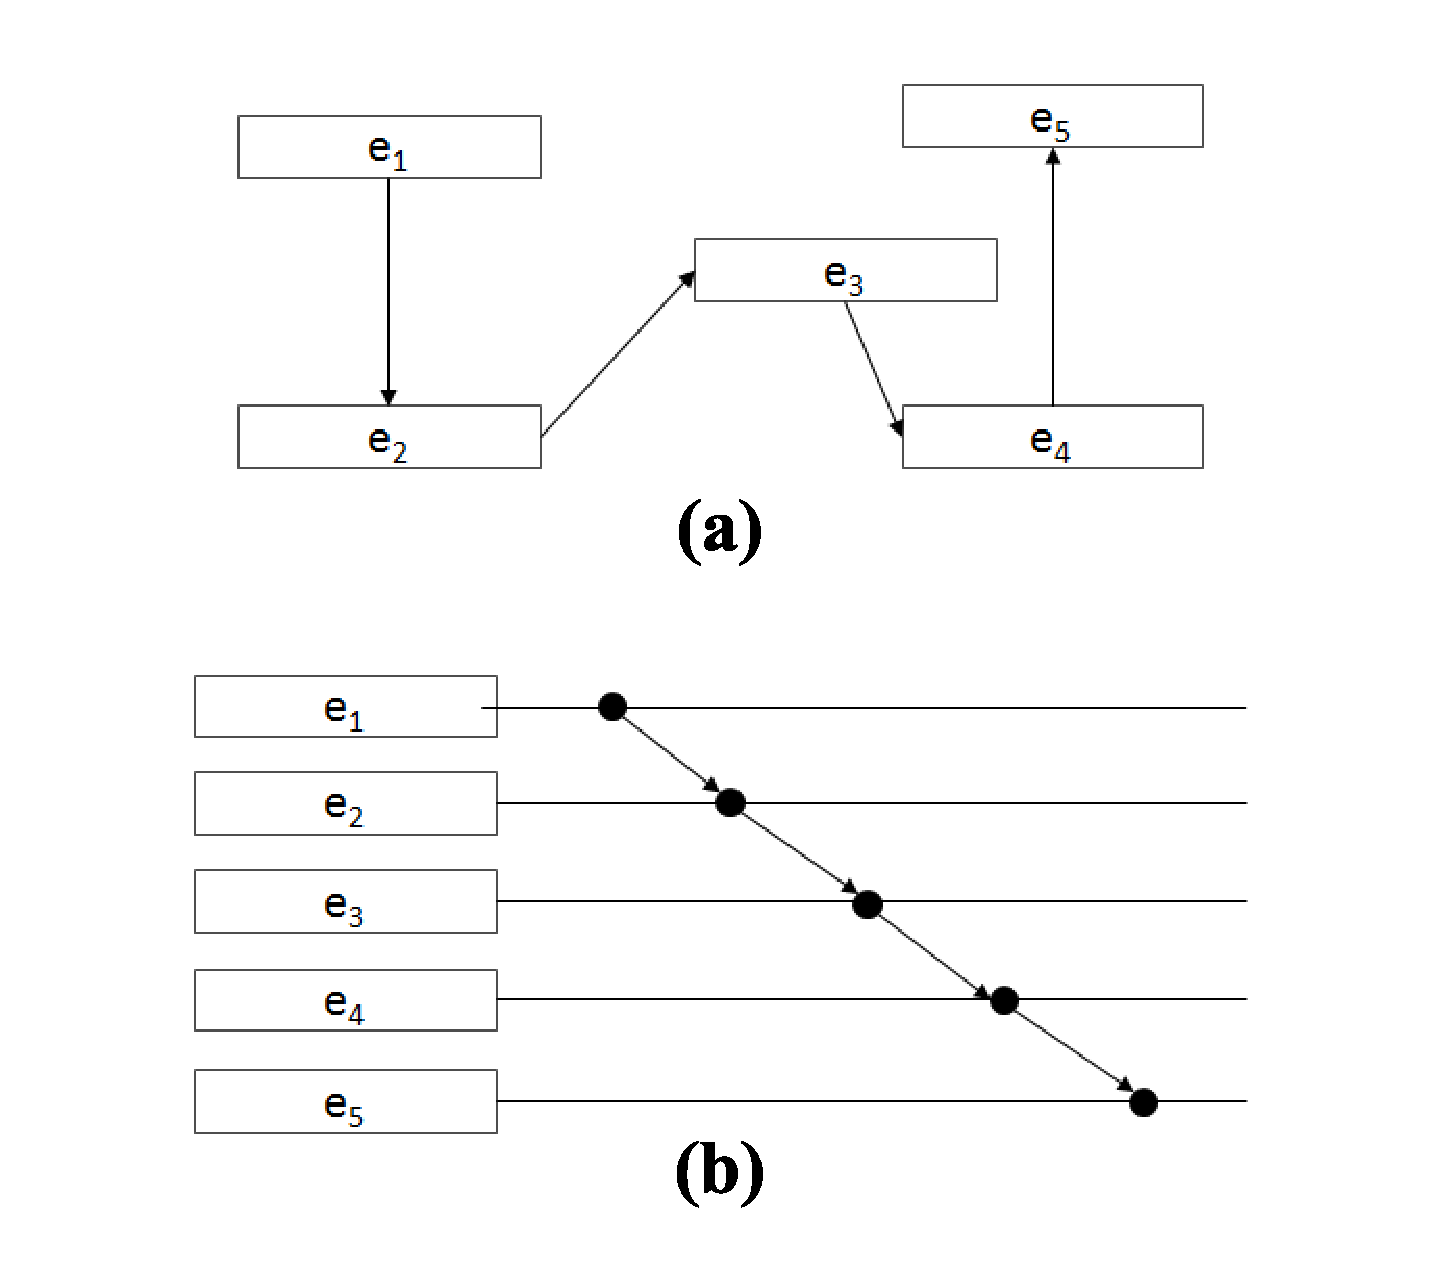
\includegraphics[width=\linewidth]{images/scanpathExample.eps}
  \caption{Scanpath visualization (a) without explicit temporal information, (b) with temporal transitions.}
	\label{fig:scanpathExample}
\end{figure}

\subsection{Scarfplot}
In a scarplot technique, visual entities are joined as multiple tapes known as scarflines~\cite{richardson2005looking}. The entities may have different width in tapes. The width usually represent data value (e.g. intensity). Figure~\ref{fig:scarfplotExample} demonstrate an example of transitions viewing pattern for two users. $User_1$ viewed entities $e_1, e_2, e_3, e_4,e_5$ and $User_2$ viewed $e_6, e_7$. Scarfplot technique is useful for finding pattern among multiple sets of data. 
\begin{figure}[htbp]
  \centering
  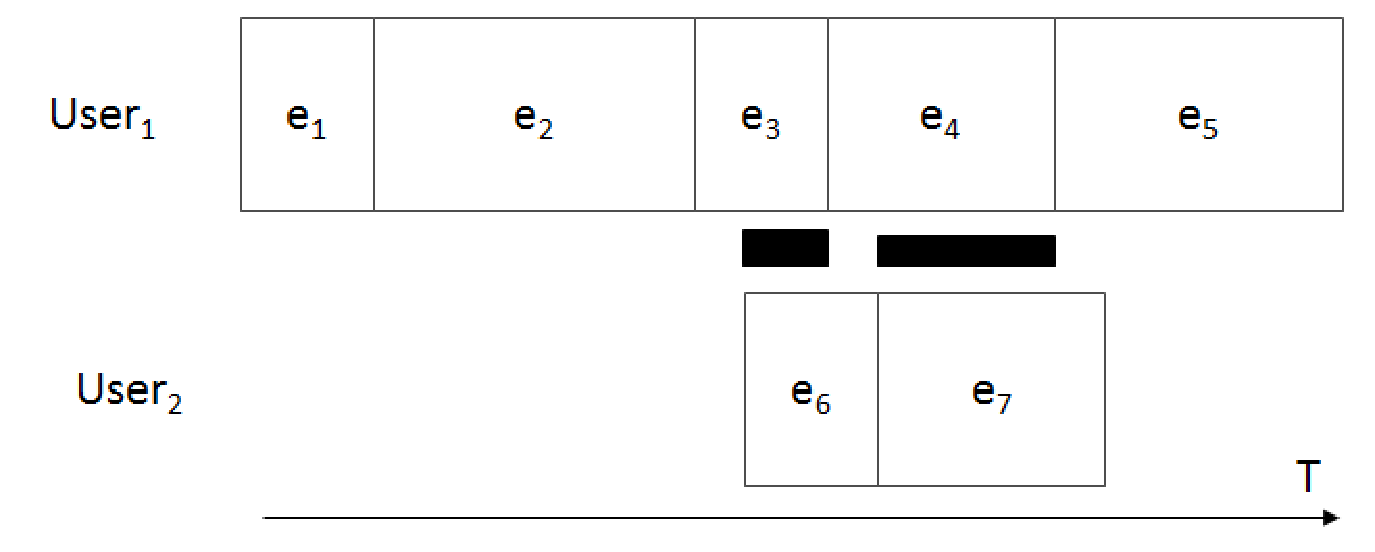
\includegraphics[width=\linewidth]{images/ScarfplotExample.eps}
  \caption{An example of Scarfplot visualization. }
	\label{fig:scarfplotExample}
\end{figure}

\section{Case Studies}
In this section, we discuss our implementation of four DOI analysis visualizations: heatmap, scanpath, scarfplot, and stacked glyph-plot. We developed these visualizations based on collected DOI data from experiments in Chapter~\ref{chap:CaseStudies}. Specifically, we generated for the study described in Section~\ref{sec:ExperimentIMDB}. Next, we developed another heatmap for the study described in Section~\ref{sec:ExperimentArchitecture}, and a stacked glyph plot for the experiment described in Section~\ref{sec:ExperimentConstruction}. We discuss more of them below. 

\subsection{DOI-Vis for the Tracking Data Consumption Experiment}
We already discussed the data collection and instrumentation methods about the tracking data consumption experiment in Section~\ref{sec:ExperimentIMDB}. To analyze the data collected from this study, we developed three visualizations: heatmap, scanpath, and scarfplot. 

First, we developed a time-annotated heatmap (Figure~\ref{fig:HeatmapIMDB}) where each cell's color represents viewing score (i.e. viewing-intensity). We chose the grayscale color scheme to render the heatmap where black represents maximum and white represents the minimum. In our visualization, we facilitate interaction of panning to view time-based data. For facilitating comparison, we allowed rendering user data views side by side. 
\begin{figure}[htb]
  \centering
	\includegraphics[width=0.75\linewidth]{images/HeatmapIMDB.eps}
  \caption{An example of a heatmap generated from real DOI data. It shows user-data separately. DOI-rows are scaled vertically to make often viewed DOIs more salient. The visualization orders DOIs by viewing-score and do not display the DOIs with viewing-scores are beyond a threshold. A time-window (white section) helps prioritize for selecting which data to show.}
	\label{fig:HeatmapIMDB}
\end{figure}

Second, we have implemented a scanpath for the same experiment (Figure~\ref{fig:ScanpathsIMDB}). Unlike heatmap, we considered every DOI as `viewed' when its viewing score crossed a threshold value (e.g. 0.75). Then, we connected the DOI cell to render the scanpath. The scanpath rendering had two versions: juxtaposed (Figure~\ref{fig:ScanpathsIMDB}(left)) and superpositioned(Figure~\ref{fig:ScanpathsIMDB}(right)). We applied a string edit-distance clustering over the vertical sequence of DOIs to reduce cluttering. 
\begin{figure}[!htb]
  \centering
  \includegraphics[width=0.75\linewidth]{images/ScanpathsIMDB.eps}
  \caption{Scanpaths of real DOI data. (left) Data is shown separately for each user. Depicted DOIs are the same for all four users, enabling the comparison of the scanpath profile; the top two users viewed similar data. (right) Users' data are shown next to each other for each DOI; we notice that the four users cluster into two pairs, based on their interests.}
	\label{fig:ScanpathsIMDB}
\end{figure}

\begin{figure}
  \centering
  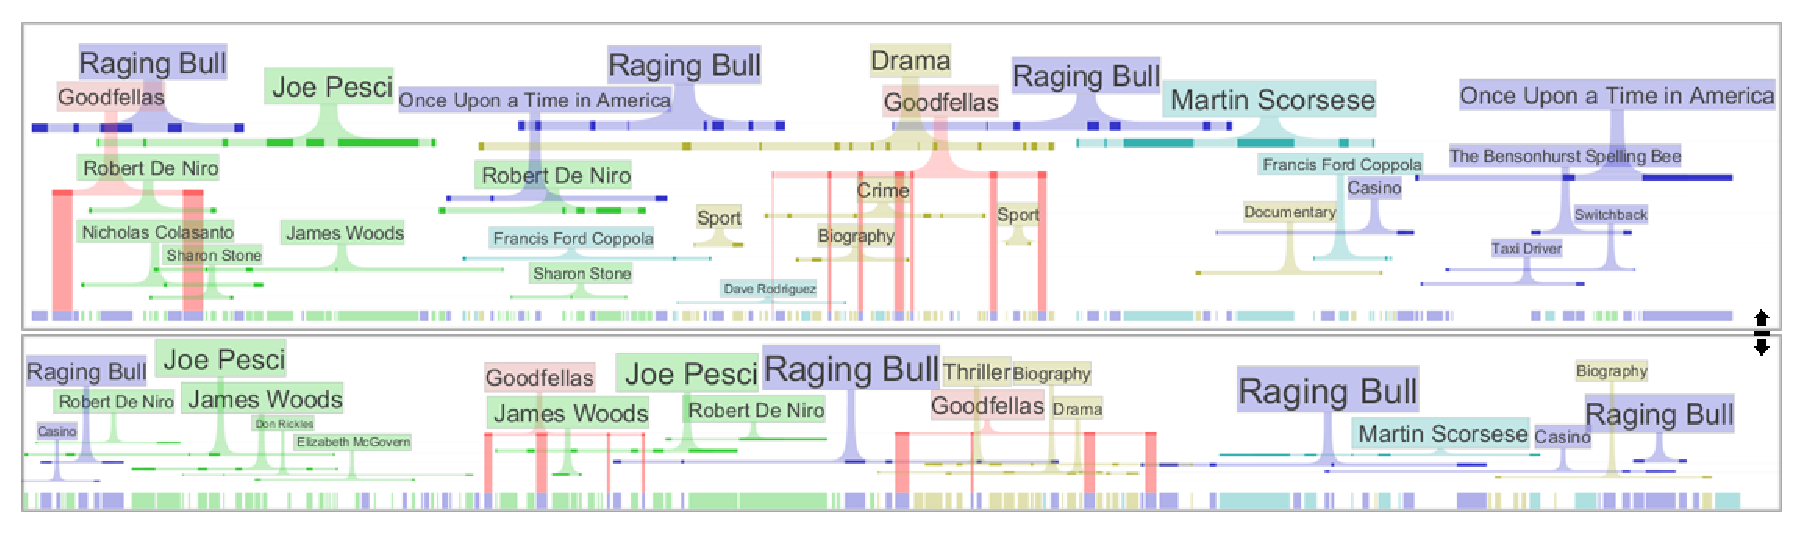
\includegraphics[width=\linewidth]{images/ScarfsIMDB.eps}
  \caption{A DOI-scarfplot for movie DOI data sketched for two users. DOI are labeled explicitly and scaled according to their viewing-score around particular time-points. Vertical resizing of a users' plot would show less or more data. The figure highlighted a selection for one user (Goodfellas) in all data. }
	\label{fig:ScarfsIMDB}
\end{figure}

Third, we modified the original scarfplot to enable DOI data visualization. We developed a scarfplot with clear labels (Figure~\ref{fig:ScarfsIMDB}. Moreover, the labels attach themselves with the scarf area on the scarflines. To support multiple granularities, we rendered many scarflines to show DOIs clearly. 
%\begin{figure}[htb]
  %\centering
	%\includegraphics[width=0.5\linewidth]{images/MatrixGraphIMDB.eps}
  %\caption{Transition matrix and graph of real DOI data. Both support multiple time-scales by allowing transitions to be defined flexibly, depending on the maximum time allowed to pass between when a first and second object are viewed. The graph shows often viewed objects larger.}
	%\label{fig:MatrixGraphIMDB}
%\end{figure}

\subsection{DOI-Vis for the Student Learning Experiment}
We developed an interactive heatmap visualization (Figure~\ref{fig:HeatmapArchitecture}) for the student learning experiment from the Section~\ref{sec:ExperimentArchitecture}. In Figure~\ref{fig:HeatmapArchitecture}, we lined up all detected DOIs on the left and their viewing timeline on the right. A sorting option for DOI lineup is also available where we can sort DOIs over first viewed, most viewed or by categories. We collected DOIs of three categories: text, navigation (i.e. buttons, links), and image AOIs. We added selection option where a pop-up dialog appears whenever we select any DOI. The pop-up dialog describes DOI details and possible image section from the original stimuli. We also enabled the timeline panel to be dragged to have a better view of DOI data. 
\begin{figure}
  \centering
  \includegraphics[width=\linewidth]{images/architecture.eps}
  \caption{An example of interactive heatmap visualization for the student learning experiment (described in Section~\ref{sec:ExperimentArchitecture}). }
	\label{fig:HeatmapArchitecture}
\end{figure}

\subsection{DOI-Vis for the Construction Hazard Detection Experiment}
We implemented a glyph-based visualization for hazard detection experiment discussed in Section~\ref{sec:ExperimentConstruction}. The visualization (Figure~\ref{fig:constructionAnalysis}) employs focus+context technique and glyph based solution to handle multiple granularities of DOI data and to handle data attributes. 

Focus$+$context is an interactive technique which is similar to overview$+$detail technique. Overview$+$detail have two sections of the involving visualization: overview and detail. In the `Overview' section, we can view the whole display with minimal readability, and the detail view shows a detail of a part of the `Detail' section. On the other hand, focus+context combines the two sections in a single coherent view~\cite{spence1982data}. Using such technique will facilitate analyzers to navigate through DOI data. 

On the other hand, a glyph is a small visual object that is discretely placed in visualizations. It is useful to depict data attributes~\cite{borgo2013glyph}. Glyph designing often combines concepts of Gestalt psychology~\cite{kohler1970gestalt}, visual channel selection, and design criteria. For example, if we want to design a glyph for $O = {a_1, a_2}$ where $a_i$ is the $i$th attribute for object $O$. We assume that the attributes are sorted in descending order of importance(i.e. $a_1$ is the most important attribute and $a_2$ is the least). We can assign four visual channels for all the attributes: color, and size. According to the pop-out effect of visual channel, color precedes size in importance. Thus, users will be able to detect whether a visual object is red or blue first then whether it is big or small. 

A suitable instance of a glyph is star-plot. A star-plot contains radially arranged multiple axes (i.e. rays)~\cite{klippel2009star}. Each attribute of involving data element corresponds to a star-plot ray. Connecting data points of each ray create a star-like shape to create such star-plot. Using star-plots for DOI data significantly facilitates handling data attribute. 

In Figure~\ref{fig:StarplotExample}, we describe an example for star plot. Suppose, we want to represent a DOI $D_1=\cup_{1 \leq i \leq N}a_i=v_i $, where $a_i$ represents $i$th attribute and $v_i$ is the value of $a_i$. We entitle a ray for each attribute $a_i$. For $v_i$ we mark a point along the ray for $a_i$. Then, we connect all the line to form a star-like shape.  
\begin{figure}[htbp]
  \centering
  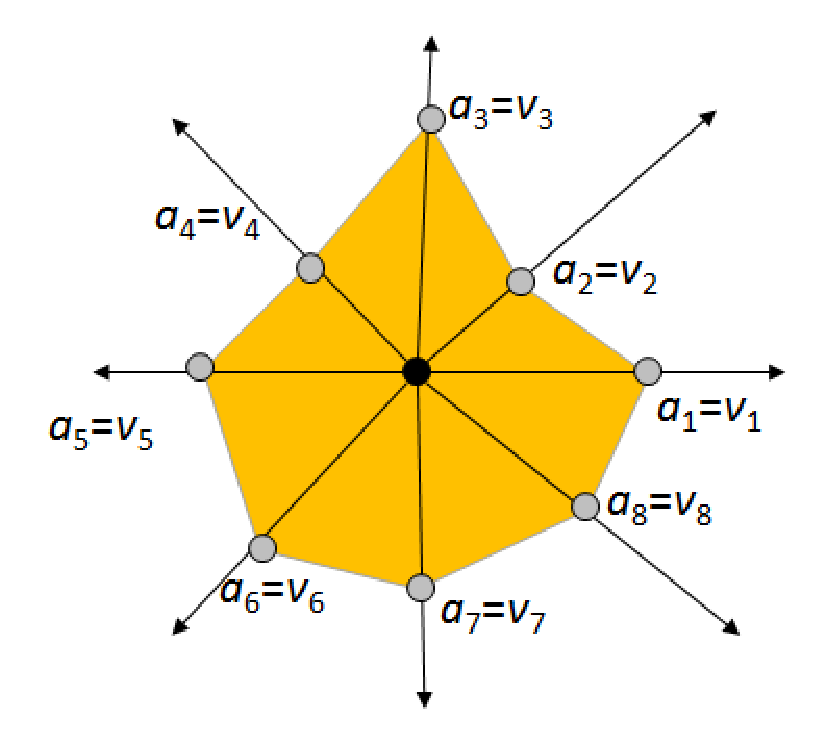
\includegraphics[width=0.5\linewidth]{images/StarplotExample.eps}
  \caption{An example of a star-plot glyph.}
	\label{fig:StarplotExample}
\end{figure}

In Figure~\ref{fig:constructionAnalysis}, we show a glyph for what type of DOI (e.g. worker) it is alongside a star plot over it. We also enabled sorting option based on data attributes. Moreover, we enabled panning and filtering. Again, we used colors to detect whether the users identified any hazard over a particular DOI and color coded them. 

\begin{figure}
  \centering
  \includegraphics[width=\linewidth]{images/constructionAnalysis.eps}
  \caption{Stacked Glyph plot for Construction}
	\label{fig:constructionAnalysis}
\end{figure}

\section{A Visual Design Space for DOI Analysis}

In this section, we analyze the design space for visual DOI analysis in more detail. Given the scale DOI data and the breadth of DOI tasks, we should augment visual encodings augmented with interaction capabilities. To ensure that our discussion captures all visual design dimensions, we ground it in Yi's taxonomy of interaction tasks~\cite{Yi07}, which includes seven categories of visual operations: Encoding, Selection, Reconfiguration, Exploration, Abstraction/Elaboration, Filtering, and Connection/Comparison~\cite{Yi07}. We will discuss new visual solutions by starting from existing AOI visualizations and describing how we may extend and redesign them to support DOI requirements. 

\subsection{Encoding}
\label{sec:Encoding}
Encoding determines how data should be shown visually~\cite{Yi07}. We discuss encoding design options and requirements of DOI visualizations below.

\textbf{Show many DOIs :} AOI visualizations such as scarfplots identify specific AOIs via distinctive colors. This method does not scale to many DOIs, and techniques that identify DOIs explicitly (e.g., through a label), such as scan-paths or transition matrices, are likely preferable. 

Also, showing all DOIs viewed in an experiment is not always possible, especially when observing data from many users. For example, a scanpath of ten users, each having viewed $100$ DOIs would have a thousand rows and be cluttered. One solution is to show only the most viewed DOIs, as done for visualizations shown in Figures~\ref{fig:ScanpathsIMDB},~\ref{fig:ScarfsIMDB},~\ref{fig:HeatmapIMDB},~\ref{fig:HeatmapArchitecture},~\ref{fig:constructionAnalysis} and to a lot DOI space that is proportional to how often they are viewed, as exemplified in Figure~\ref{fig:HeatmapIMDB}. This prioritization approach is likely appropriate as we showed in Chapter~\ref{chap:DOIDataCollection} that even though users view many DOIs during an extended analysis, they focus most of their attention on a smaller subset of them. 

Finally, DOI attributes make it possible to collapse multiple DOIs into categories to reduce the amount of information shown, as discussed in section~\ref{sec:Interaction}, Abstract/Elaborate.


\textbf{Showing DOI attributes} can be supported via conventional techniques such as linking DOI attributes to visual channels (e.g., color, shape) or by relying on glyph designs. Displaying DOI attributes can enable analysts to detect how DOIs with similar properties clusters over time visually. For such tasks to be possible, in addition to showing properties, DOIs need to be grouped based on when they were viewed or in what transitions they were involved. For example, scarf-plots inherently order DOIs by time (Figure~\ref{fig:ScarfsIMDB}), but scan-paths and transition matrices have to be clustered to group together co-viewed DOIs (Figure~\ref{fig:ScanpathsIMDB}). Additionally, showing multiple attributes for each DOI facilitates a visual approximation of attribute-derived measures, supporting summarization tasks. Figure~\ref{fig:constructionAnalysis} exemplifies showing many data attributes using glyph based designs. 


\textbf{Reducing clutter} is essential in busy DOI visualizations. Clustering is one effective way to impose order on visualizations. Figure~\ref{fig:ScanpathsIMDB} shows scanpaths that orders DOIs based on how often there are transitions between them. This in effect shortens the vertical transition in the paths. Second, linking DOI appearance to their attributes can divide DOIs into data categories or layers that are visually separable, by the Gestalt principles~\cite{kohler1970gestalt}. Third, reducing shown information using semantic zooming and DOI grouping, and highlighting and filtering, can also reduce clutter, as discussed in the next sections. 

A further factor needs to be considered when supporting analyses of DOI data from many subjects. Visualization datasets can sustain hundreds or thousands of DOIs, which subjects, based on their interests and exploration, will only see small subsets of them. These subsets may differ significantly between subjects, leading to a tradeoff: should visualizations be optimized to best show a single user's behavior, or to show a user's behavior in the context of other users' data? The scanpaths in Figure~\ref{fig:ScanpathsIMDB} show DOIs that were viewed by all subjects, and use the same DOI-set and ordering for each user. Alternatively, each subjects' scan-path could also show and order DOIs based solely on that subject's data. The former approach shows less relevant data for each user but makes it easy to compare user behavior, while the latter would show more relevant data for each user but would hinder comparison. Similarly, scanpaths can be separate or integrate individual users' data as shown in Figure~\ref{fig:ScanpathsIMDB}, making it easier or harder to compare subjects.

\subsection{Interaction}
\label{sec:Interaction}

\textbf{Selections} allow users to track interesting objects by marking them~\cite{Yi07}. On selection targets, DOI methods support selections of DOIs, DOI categories, users, and time intervals.  As for methods of selection, two options are possible: `in situ' selections of DOIs shown in the visualization, and query-based selections of DOIs by attribute values. Finally, selected items should be highlighted visually, and brushing-and-linking should translate selections over multiple views, supporting connect and compare interactions. Figures~\ref{fig:ScanpathsIMDB},~\ref{fig:ScarfsIMDB},~\ref{fig:HeatmapIMDB},~\ref{fig:HeatmapArchitecture} exemplify DOI selections, time-window selections, and brushing and linking.

\textbf{Reconfigurations} change the spatial arrangement of data.  In section~\ref{sec:Encoding} we already discussed the benefit of clustering co-viewed DOIs to reduce clutter and to support the detection of correlations between DOI categories and their viewing time. Additionally, DOIs should be orderable based on their attributes. Similarly, clustering and arranging subjects by their behavior can create more organized visualizations, while the ability to cluster subjects on their background or demographic data (e.g., expert vs. naive subjects) can support tasks typical of human experimentation. Finally, visualizations should also support interactive repositioning (e.g., of users, DOIs), to allow analysts to arrange and group items manually.


\textbf{Exploration} enables users to analyze different subsets of data instances. DOI data visualizations should support time-scrolling, panning, and zooming efficiently. Exploration options also include the ability to flexibly define which DOI attributes should be mapped visually, given that the number of variables that can be visually encoded concurrent may be limited. 
	
\textbf{Abstract/Elaborate} interactions allow users to control a visualization's level of abstraction. Our discussion on encoding emphasizes the need for representations that support analyses at multiple time-scales, DOI grouping, and the ability to control the amount of data shown. 

First, semantic zooming can be an efficient way to explore different time scales and involves aggregating and summarizing data over variable time-steps (e.g., milliseconds to minutes). An alternative to semantic zooming is pixel-based techniques which allow individual viewing events to merge and blend visually\cite{keim2000designing}. The re-imagined scarfplot design in Figure~\ref{fig:ScarfsIMDB} exemplifies the first approach by grouping co-viewed elements together, while the heatmap in Figure~\ref{fig:heatmap}, the second. The stacked glyph plot Figure~\ref{fig:constructionAnalysis} also exemplify semantic zooming by providing the ability to adjust the data granularity used for detail viewing interactively.  

Second, we can group DOIs by using attribute queries to define DOI categories, by exploiting DOI hierarchies (i.e., DOIs that are contained by other DOIs), or manually. Aggregating DOIs visually can again be done semantically, by allowing analysts to collapse multiple DOIs into single ones explicitly, or by showing data in a way that allows categories to emerge and separate visually (Figure~\ref{fig:constructionAnalysis}). 

Finally, details on demand can give access to additional data via tool-tips and auxiliary information data panels, populated with data obtained through brushing and linking.
  
	
\textbf{Filtering} enables users to change the set of data items being presented based on specific conditions, and should be possible on all selectable data categories previously mentioned. DOIs should be hidden or revealed based on their attributes, their viewing frequencies, viewing timestamps, and viewing users (e.g., ``Show only DOIs that both of two selected users viewed'').

We can control the number of DOIs shown directly (e.g., ``Show top $25\%$ most viewed data''), or by adjusting the amount of space allotted to users and filling it with as much data as can fit, as suggested in Figure~\ref{fig:ScarfsIMDB}. The latter is a useful way of controlling the amount of information based on available screen space and how many users or time-intervals one needs to compare.

Defining time-windows of interest can support both reconfiguration and filtering interactions. DOI visualizations will likely need to prioritize which data to show. Thus,  defining such configuration based specific time windows can answer DOI analysis questions. For example, by prioritizing the display of data that subjects viewed late in an experiment, an analyst could un-clutter the visualization of data which subjects viewed during preliminary exploration and search processes, and more clearly reveal how final data interests crystallize.

\textbf{Connection/Comparison} interactions show associations and relationships between data items and can be implemented using one of Gleicher et al.'s visual comparison methods: juxtaposition, superposition, and encoding of differences~\cite{Glei11}.In juxtaposition, two visualization placing side by side facilitate comparison. Next, in superposition, we can render one visualization over another to aid similarity among them. Finally, in explicit encoding, we can describe explicit relationship visually by encoding two data in a single view.

Visual analyses are not limited to the categories as mentioned earlier. Besides, the three types are the basic categories. We can generate hybrid categories from them. In Figure~\ref{fig:ComparisonCategories}, we describe an example of two user data $User_1$ and $User_2$. Figure~\ref{fig:ComparisonCategories}(i) depicts comparison by juxtaposing them, by superpositioning them in Figure~\ref{fig:ComparisonCategories}(ii). Figure~\ref{fig:ComparisonCategories}(iii) depicts a specific encoding of intersection between them.  
\begin{figure}[htbp]
  \centering
  \includegraphics[width=0.75\linewidth]{images/ComparisonCategories.eps}
  \caption{An example of comparison categories by Gleicher et al.~\cite{Glei11}. i) Juxtaposition, ii)Superposition, and iii) Explicit encoding (Intersection).}
	\label{fig:ComparisonCategories}
\end{figure}

To support juxtaposition, an ideal visualization should show data from multiple users or from multiple time intervals using compact, stackable, and comparable visualizations. The designs in Figures~\ref{fig:ScanpathsIMDB},~\ref{fig:ScarfsIMDB},~\ref{fig:HeatmapIMDB},~\ref{fig:HeatmapArchitecture}, and~\ref{fig:constructionAnalysis} can be resized to show more or less of a user's data, to multiple user-views to fit in a single screen, and the scanpaths use the same DOI ordering for all users to support comparison. Superposition is exemplified in the right panel of Figure~\ref{fig:ScanpathsIMDB}. Selecting and highlighting overlaps and differences (e.g., ``Show DOIs viewed by all participants'', ``Show DOIs that are unique to a subject'') can implement the third method of comparison. Brushing and linking across users and across time would support all comparison and correlation tasks.

Finally, clustering can reveal similarities between users or time-intervals computationally. AOI sequences of multiple users have previously been clustered using a string-edit-distance~\cite{Kur14}. This gave good results for short, highly constrained perceptual tasks with few AOIs. However, this distance measure may not be robust enough to handle DOI data collected over long, open-ended tasks, since such data is not temporally aligned and is bound to differ at the key-hole level that string-editing operates. Instead, comparing users in the space of derived features (e.g., DOIs they viewed most, common DOI transitions or sequences) may be more robust to local differences. It may also allow features to be included in and excluded from a distance measure, thus enabling an exploration of which features explain observed behavior.



%\section{Evaluation}
%Construction
\section{Conclusion}
Visual interpretation of DOI data is significantly vital for DOI-based eye-tracking data analysis. In this chapter, we provided possible visualization and interaction techniques based on the existing solutions in the literature. Moreover, we have discussed challenges for visually interpreting DOI data and their solutions. 

\chapter{CONCLUSIONS}
\label{chap:Conclusion}
DOIs are subsets of data that a visual interface shows to a user. We define them in the data model underlying a visualization, by instrumenting the code that translates concrete data into visual representations. Once a visual interface instrumented, user gaze coordinates provided by an eye-tracker can be mapped to DOIs via their visual representations automatically and effortlessly, regardless of users' individual interactions with the interface. As such, the DOI approach can capture users' data interests from interactive visualizations over extended periods of time. Moreover, DOIs are characterized by a rich set of attributes derived from the data that the DOIs are defined on, and from the visual context in which they are displayed. These attributes allow analysts to pose a broad range of questions that relate the type of viewed data to user behavior and characteristics. While DOIs can be regarded as a mere extension of AOIs, there are significant differences in DOI data properties and how it is collected, the research goals it can support, and the data questions it facilitates. Moreover, current visualization techniques do not support DOI-specific analyses. These differences, detailed throughout the paper, justify the different nomenclature and motivate the research.    

DOI data can enable data-driven, exploratory eye-tracking research not previously possible, by supporting long ``in vivo'' experiments of complex and interactive visual content. To unlock these benefits, new visualization designs need to be developed. These need to handle the large scale typical of DOI data, show and leverage the rich attribute set that can characterize each DOI, and support DOI specific tasks. The dissertation creates a foundation for such research by formalizing DOI data and tasks and identifying immediate challenges in supporting DOI analyses.

% Thesis epilogue

\bibliographystyle{alpha}
\bibliography{bib}

%\appendix
%\input{appendixA}

\begin{vita}
\begin{center}
SAYEED SAFAYET ALAM \\[4ex]
\end{center}

\noindent
\begin{tabular}{ll}
November 5, 1987 & Born, Dhaka, Bangladesh \\[2ex]

2004--2009 \hspace{0.75in}         & B.S., Computer Science and Engineering \\
                                	        & Bangladesh University of Engineering and Technology \\
                                		& Dhaka, Bangladesh \\[2ex]              

2013--2017      & Doctoral Candidate \\
                    & Florida International University \\
            		& Miami, Florida \\[2ex]
\end{tabular}
\newline
\newline


\noindent
PUBLICATIONS\\[1ex]
\vspace{-5mm}

\noindent
\begin{tabularx}{\textwidth}{X}
\bibentry{AJ17}.\\\\
\bibentry{Ala16}.\\\\
\bibentry{alam2015they}.\\\\
\bibentry{alam2014data}.\\\\
\bibentry{Okoe14}.\\\\
\bibentry{okoe2013using}.\\\\
\end{tabularx}


\end{vita}



\end{document}


